%---------------------导言区---------------------------%
\documentclass[12pt,a4paper,UTF8]{ctexart}
	%10pt:正文字体为12pt,缺省为10pt;各层级字体大小会根据正文字体自动调整
	%a4paper:纸张大小a4;
	%UTF8:中文要求
\CTEXsetup[format={\Large\bfseries}]{section}
\usepackage{geometry}%用于设置上下左右页边距
	\geometry{left=2.5cm,right=2.5cm,top=3.2cm,bottom=2.8cm}
\usepackage{xeCJK,amsmath,paralist,enumerate,booktabs,multirow,graphicx,subfig,setspace,listings,lastpage,hyperref}
	%xeCJK:中文字体(如楷体,作者和机构需要用到)的设置
	%amsmath:数学公式
	%paralist,enumerate:自定义项目符号
	%booktabs:三线图,论文常用的表格风格
	%multirow:复杂表格
	%graphicx,float: 插入图片
	%subfig:并排排版图片、竖向排版图片
	%setspace:设置行间距等功能
	\setlength{\parindent}{2em}%正文首行缩进两个汉字
	%listings:用于排版各种代码;比如matlab的代码
	\lstset{language=Matlab}%matlab代码
	%lastpage:获取总页数;
	%hyperref:超链接,和lastpage搭配.
\usepackage{fancyhdr}
	%fancyhdr:一个很强大的宏包,用于自定义设计页面风格并命名以供调用。
	\pagestyle{fancy}
	\rhead{实验B1 光电效应实验}
	\lhead{基础物理实验\uppercase\expandafter{\romannumeral2}实验报告}
	\cfoot{Page \thepage/\pageref{LastPage}}  %当前页\总页数
	\rfoot{\today}
		%分别是右页眉、左页眉、中页脚、右页脚
	\renewcommand{\headrulewidth}{0.4pt}
	\renewcommand{\theenumi}{(\arabic{enumi})}

% \setCJKmainfont{FZShuSong-Z01S}[ItalicFont=FZKai-Z03S, BoldFont=FZHei-B01S]
%中文字体设置:使用开源字体方正书宋,方正楷体和方正黑体



%%%%%%%%%%%%%%%%%%%%%%%%%%%%%%%%%%%%%%%%%%%%%%%%%%%%%%%%%%
%%%%%%%%%%%%%%%%%%%%%%%%%正文开始%%%%%%%%%%%%%%%%%%%%%%%%%%
%%%%%%%%%%%%%%%%%%%%%%%%%%%%%%%%%%%%%%%%%%%%%%%%%%%%%%%%%%

\begin{document}

%%begin-------------------标题与信息-----------------------%%

%%标题
\begin{center}
\LARGE\textbf{实验B1 光电效应实验}
\end{center}


%%end-------------------标题与信息-----------------------%%


\section*{【数据处理与分析】}
\subsection*{一、测量普朗克常数}
\subsubsection*{1.零电流法计算普朗克常数}
\begin{figure}[htbp]
	\centering
	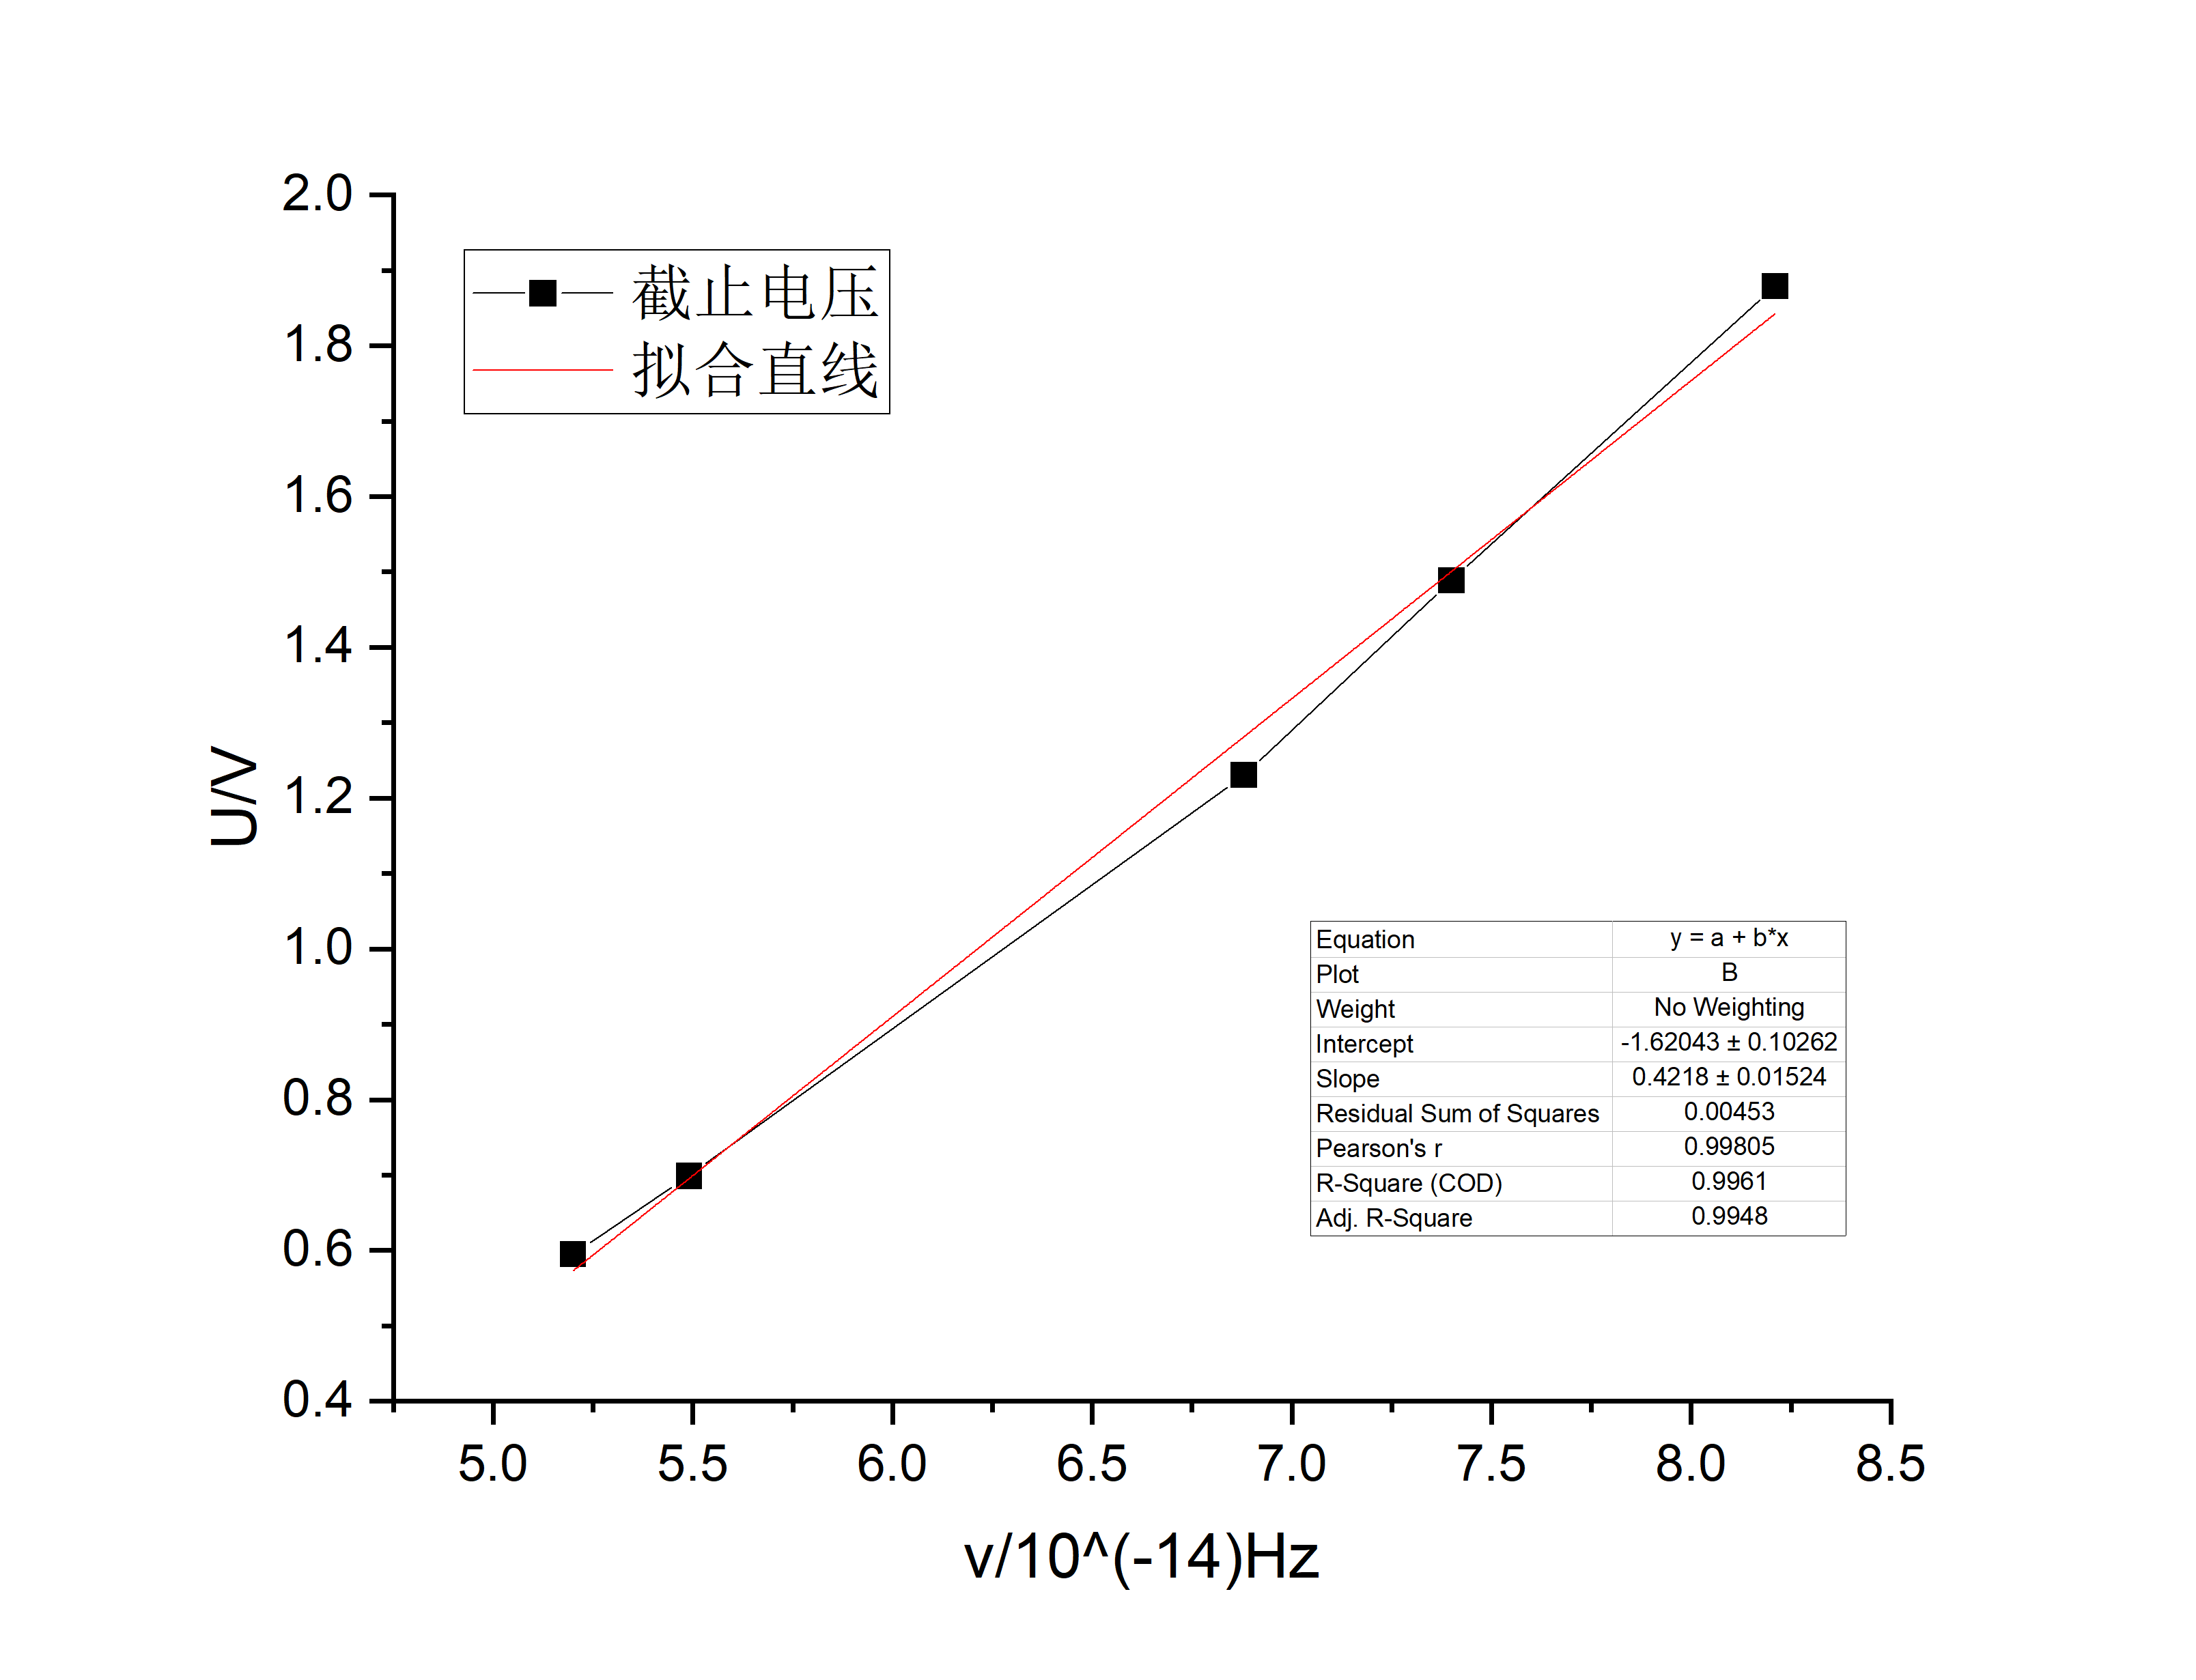
\includegraphics[width=0.6\textwidth]{img//reg.png}
	\caption{截止电压随光源频率的变化曲线}
	\label{fig:1}
\end{figure}

如图\ref{fig:1},利用最小二乘法对数据进行拟合得斜率$k=0.4218\times 10^{-14}$,
由公式
\begin{equation*}
	eU_s=h\nu-W_s
\end{equation*}

可知斜率$k=\frac{h}{e}$.
取元电荷标准值$e=1.6\times 10^{-19}C$可求得普朗克常数:
\begin{equation*}
	h=ke=6.75\times10^{-34} J \cdot s
\end{equation*}

查得普朗克常数标准值$h_0=6.63\times10^{-34} J \cdot s$,计算相对误差E:
\begin{equation*}
	E=\frac{\left\lvert h-h_0\right\rvert }{h_0}\times 100\%=1.8\%
\end{equation*}

\subsubsection*{2.用抬头点计算普朗克常数}
\begin{figure}[htbp]
	\centering
	\subfloat[$\lambda=365nm$]{\label{fig:365}
	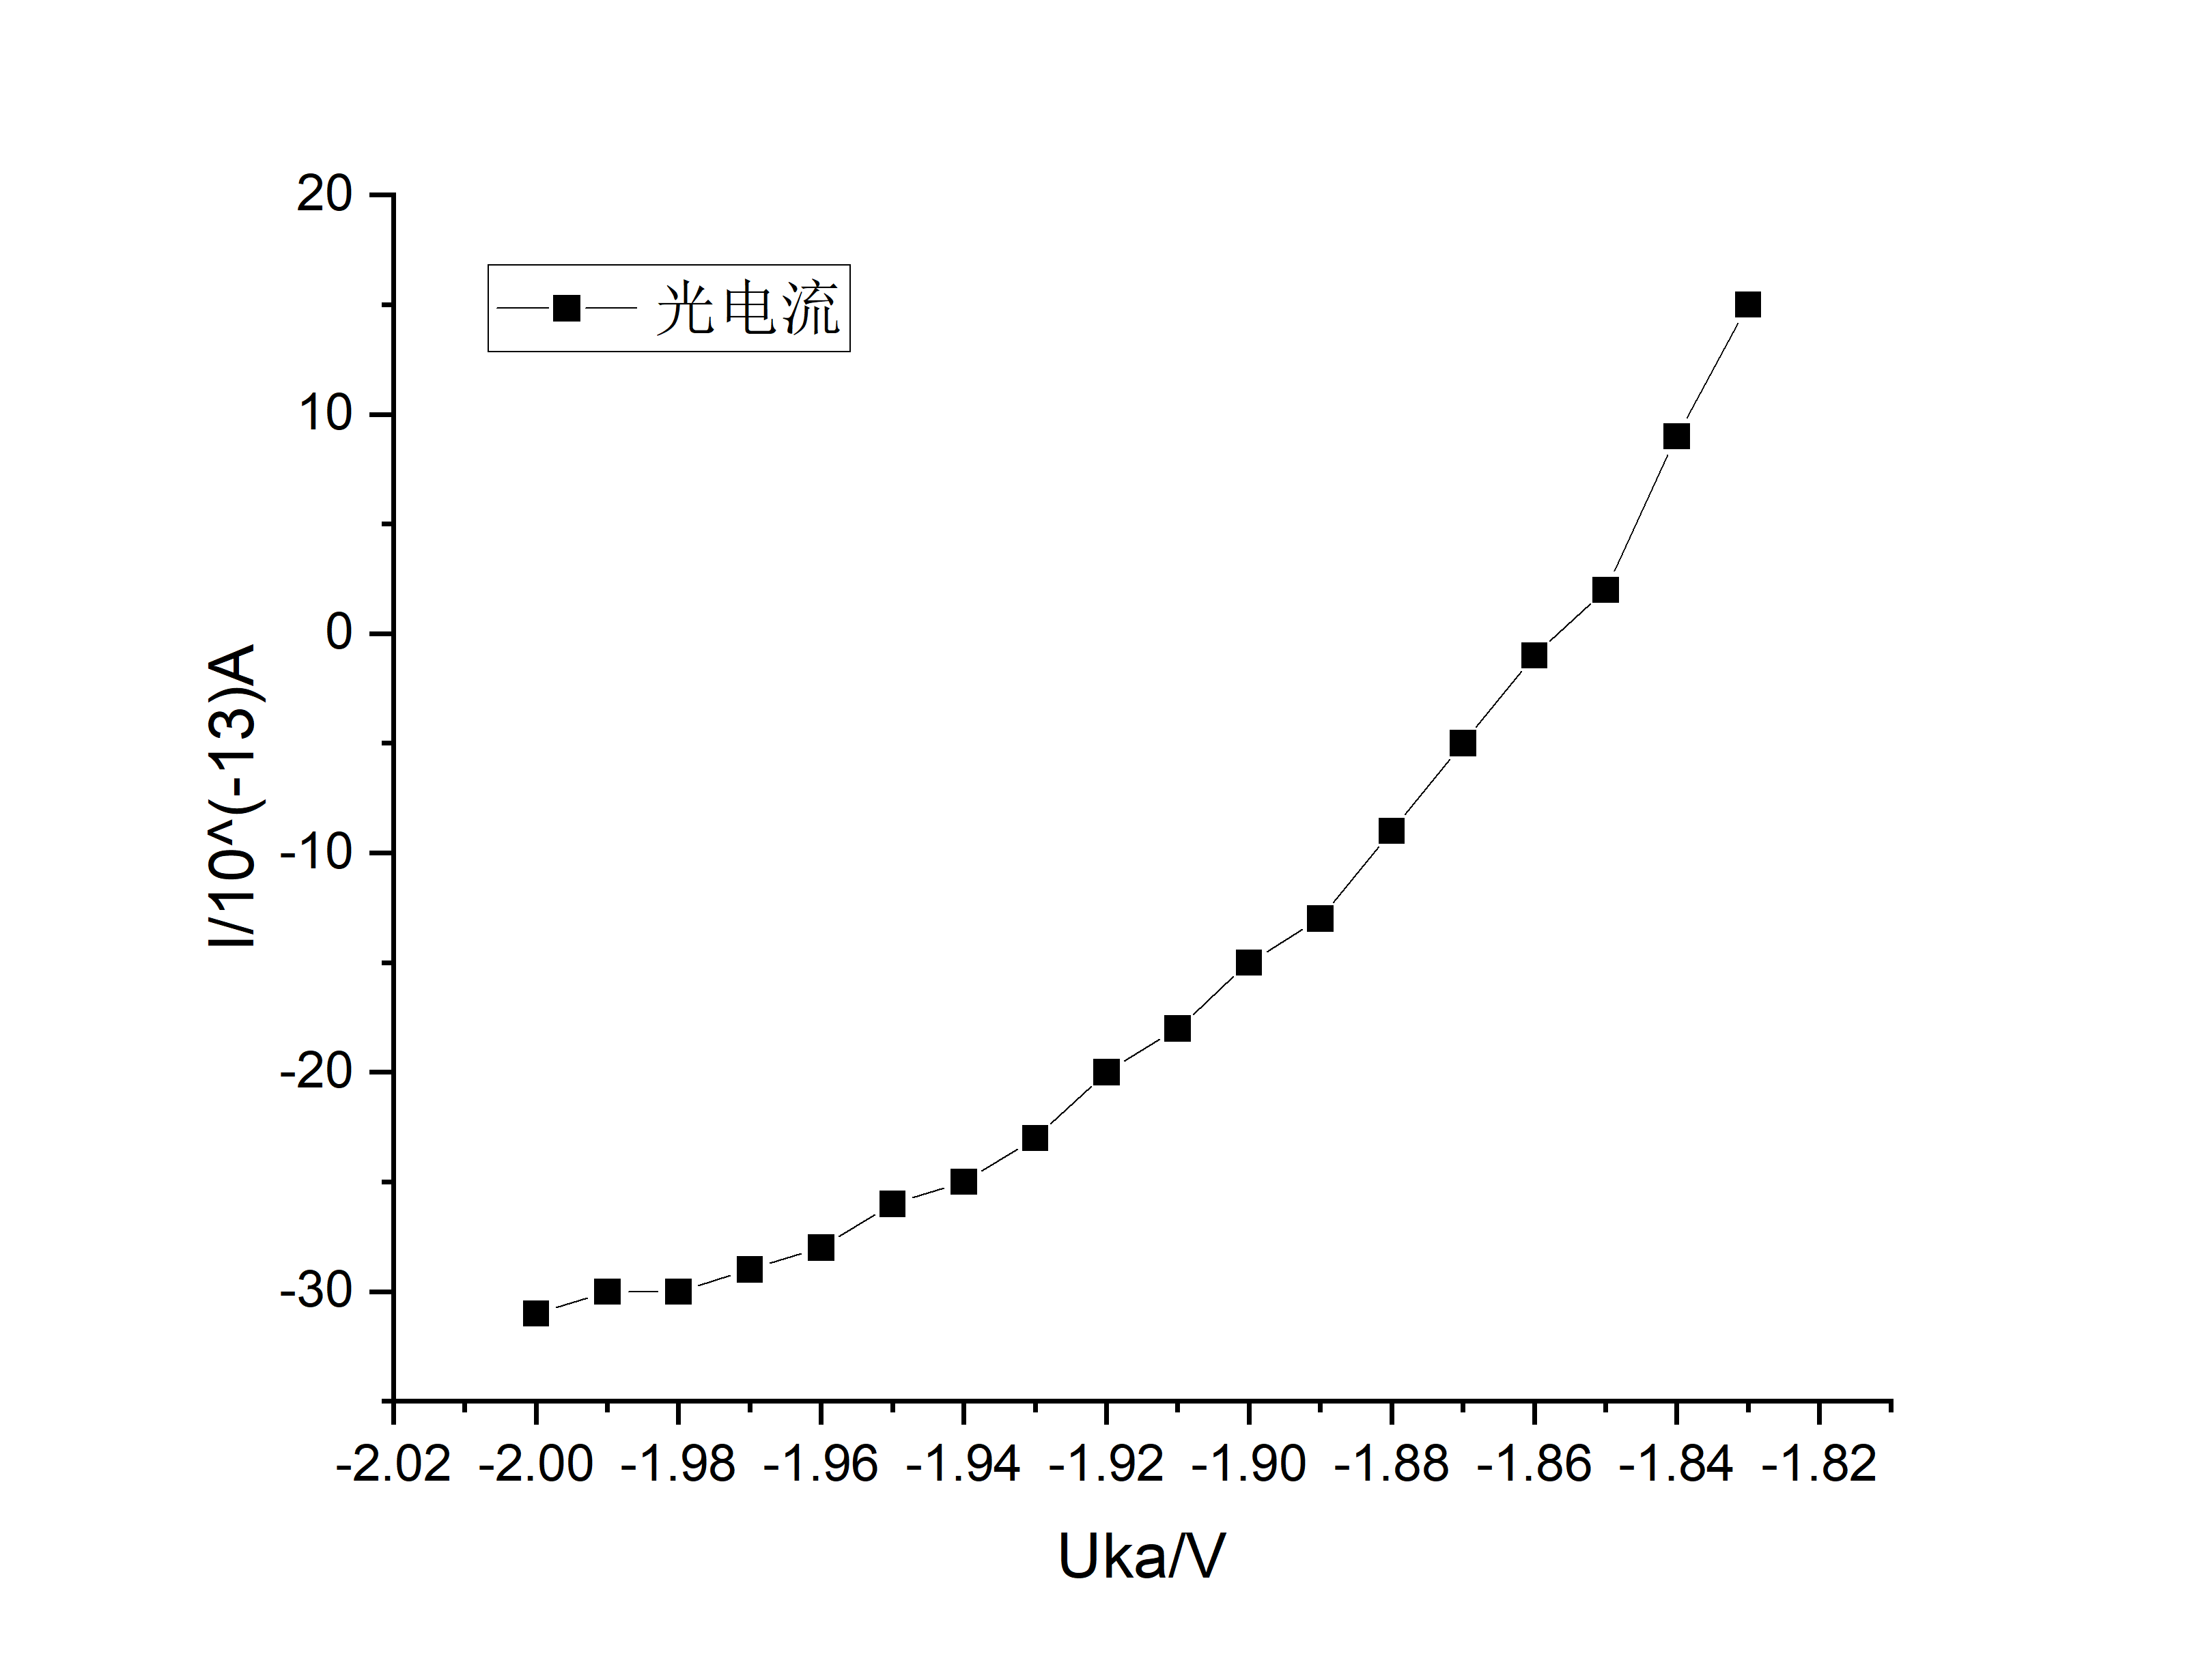
\includegraphics[width=0.33\textwidth]{img//365.png}
	}
	\subfloat[$\lambda=405nm$]{\label{fig:405}
	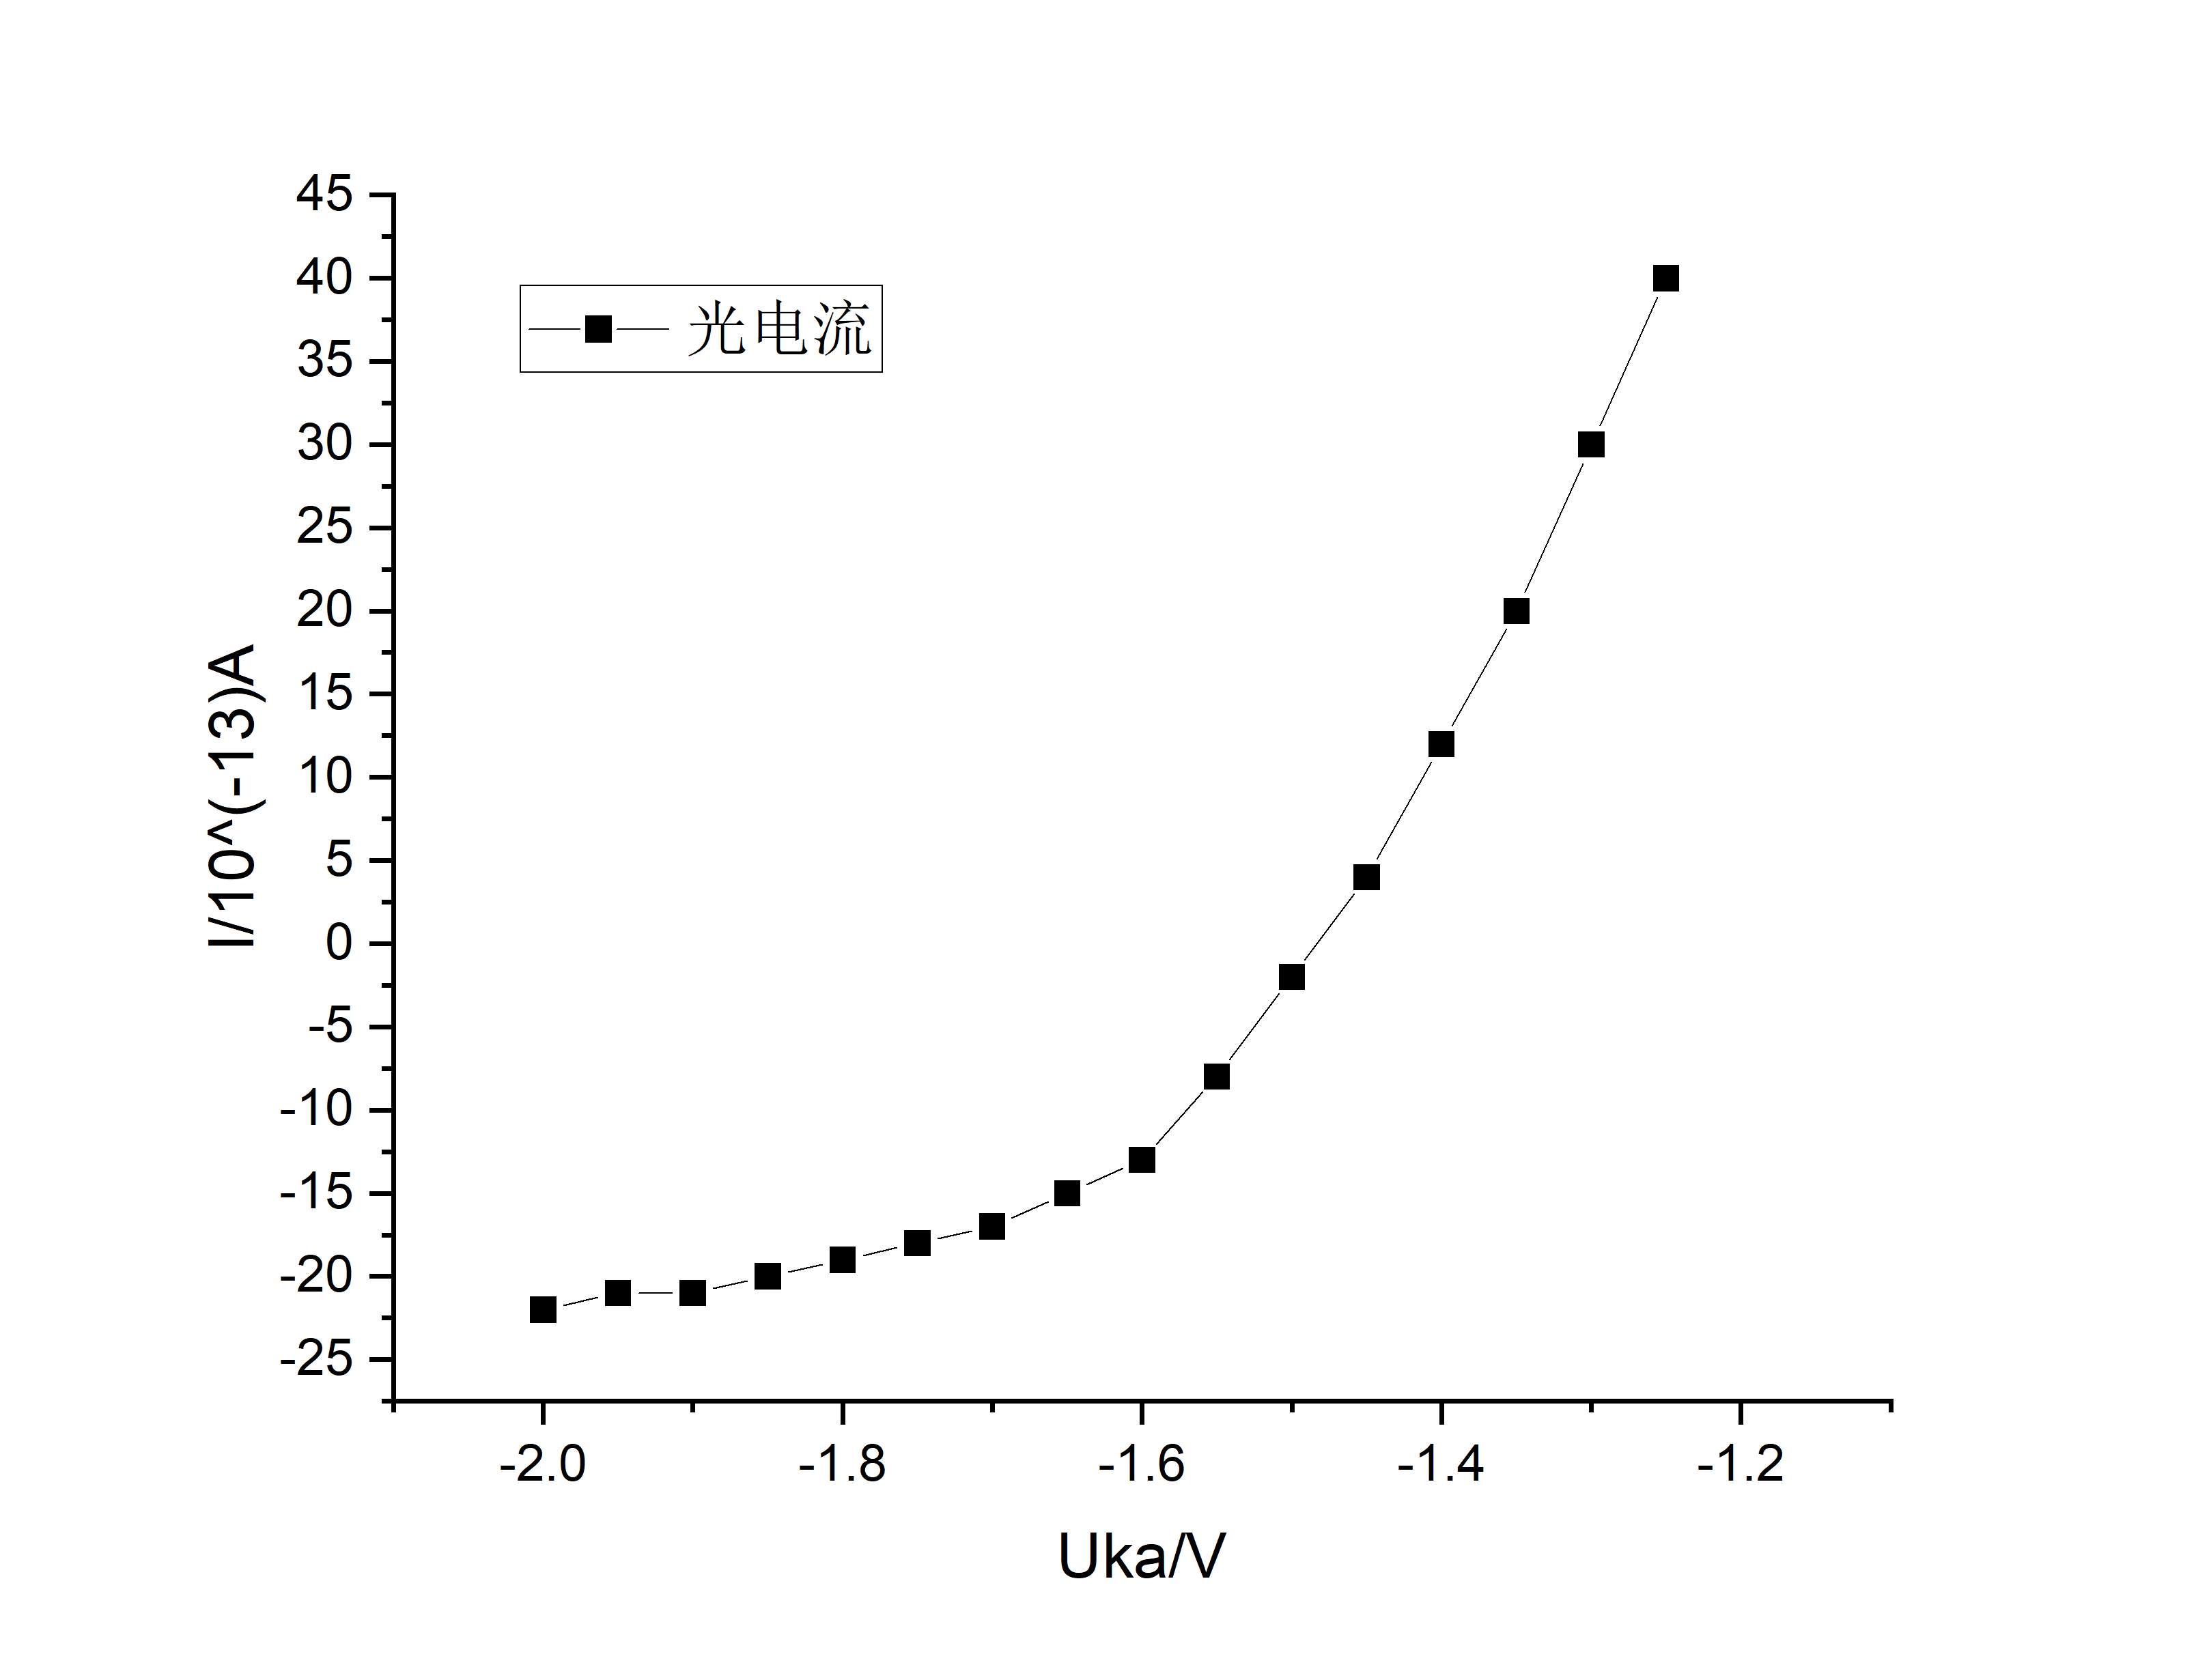
\includegraphics[width=0.33\textwidth]{img//405.png}
	}
	\subfloat[$\lambda=436nm$]{\label{fig:436}
	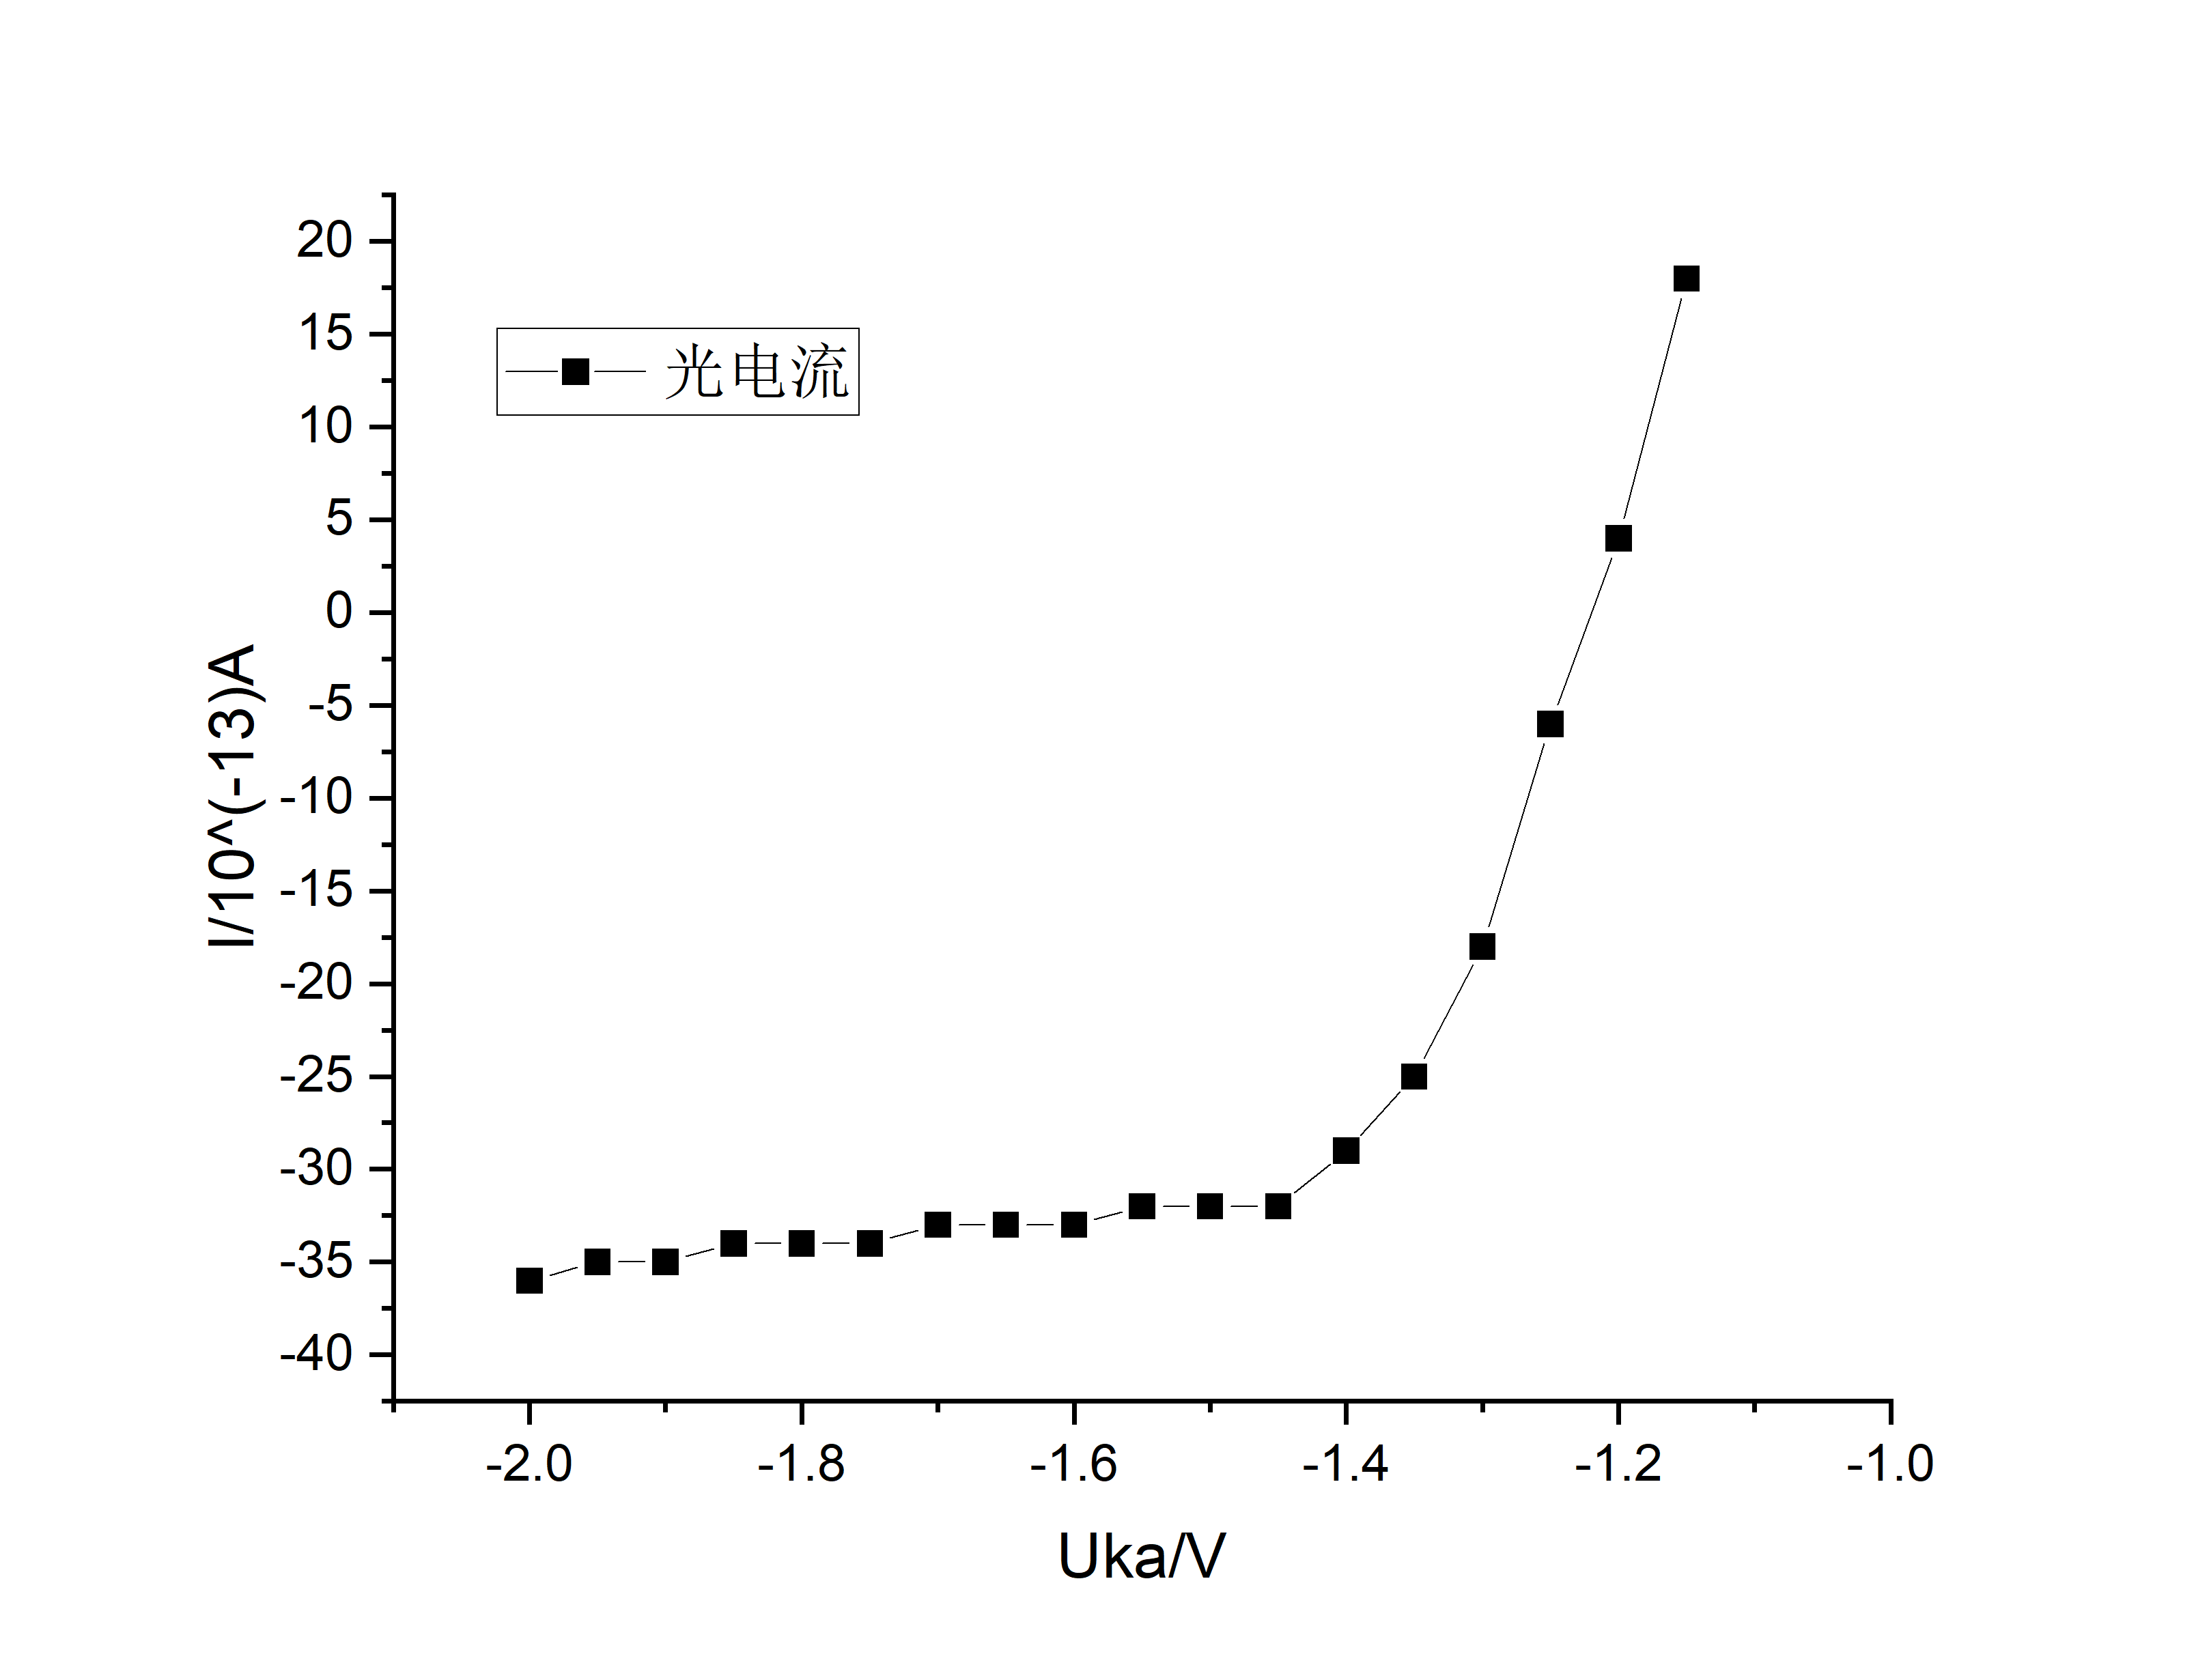
\includegraphics[width=0.33\textwidth]{img//436.png}
	}

	\subfloat[$\lambda=546nm$]{\label{fig:546}
	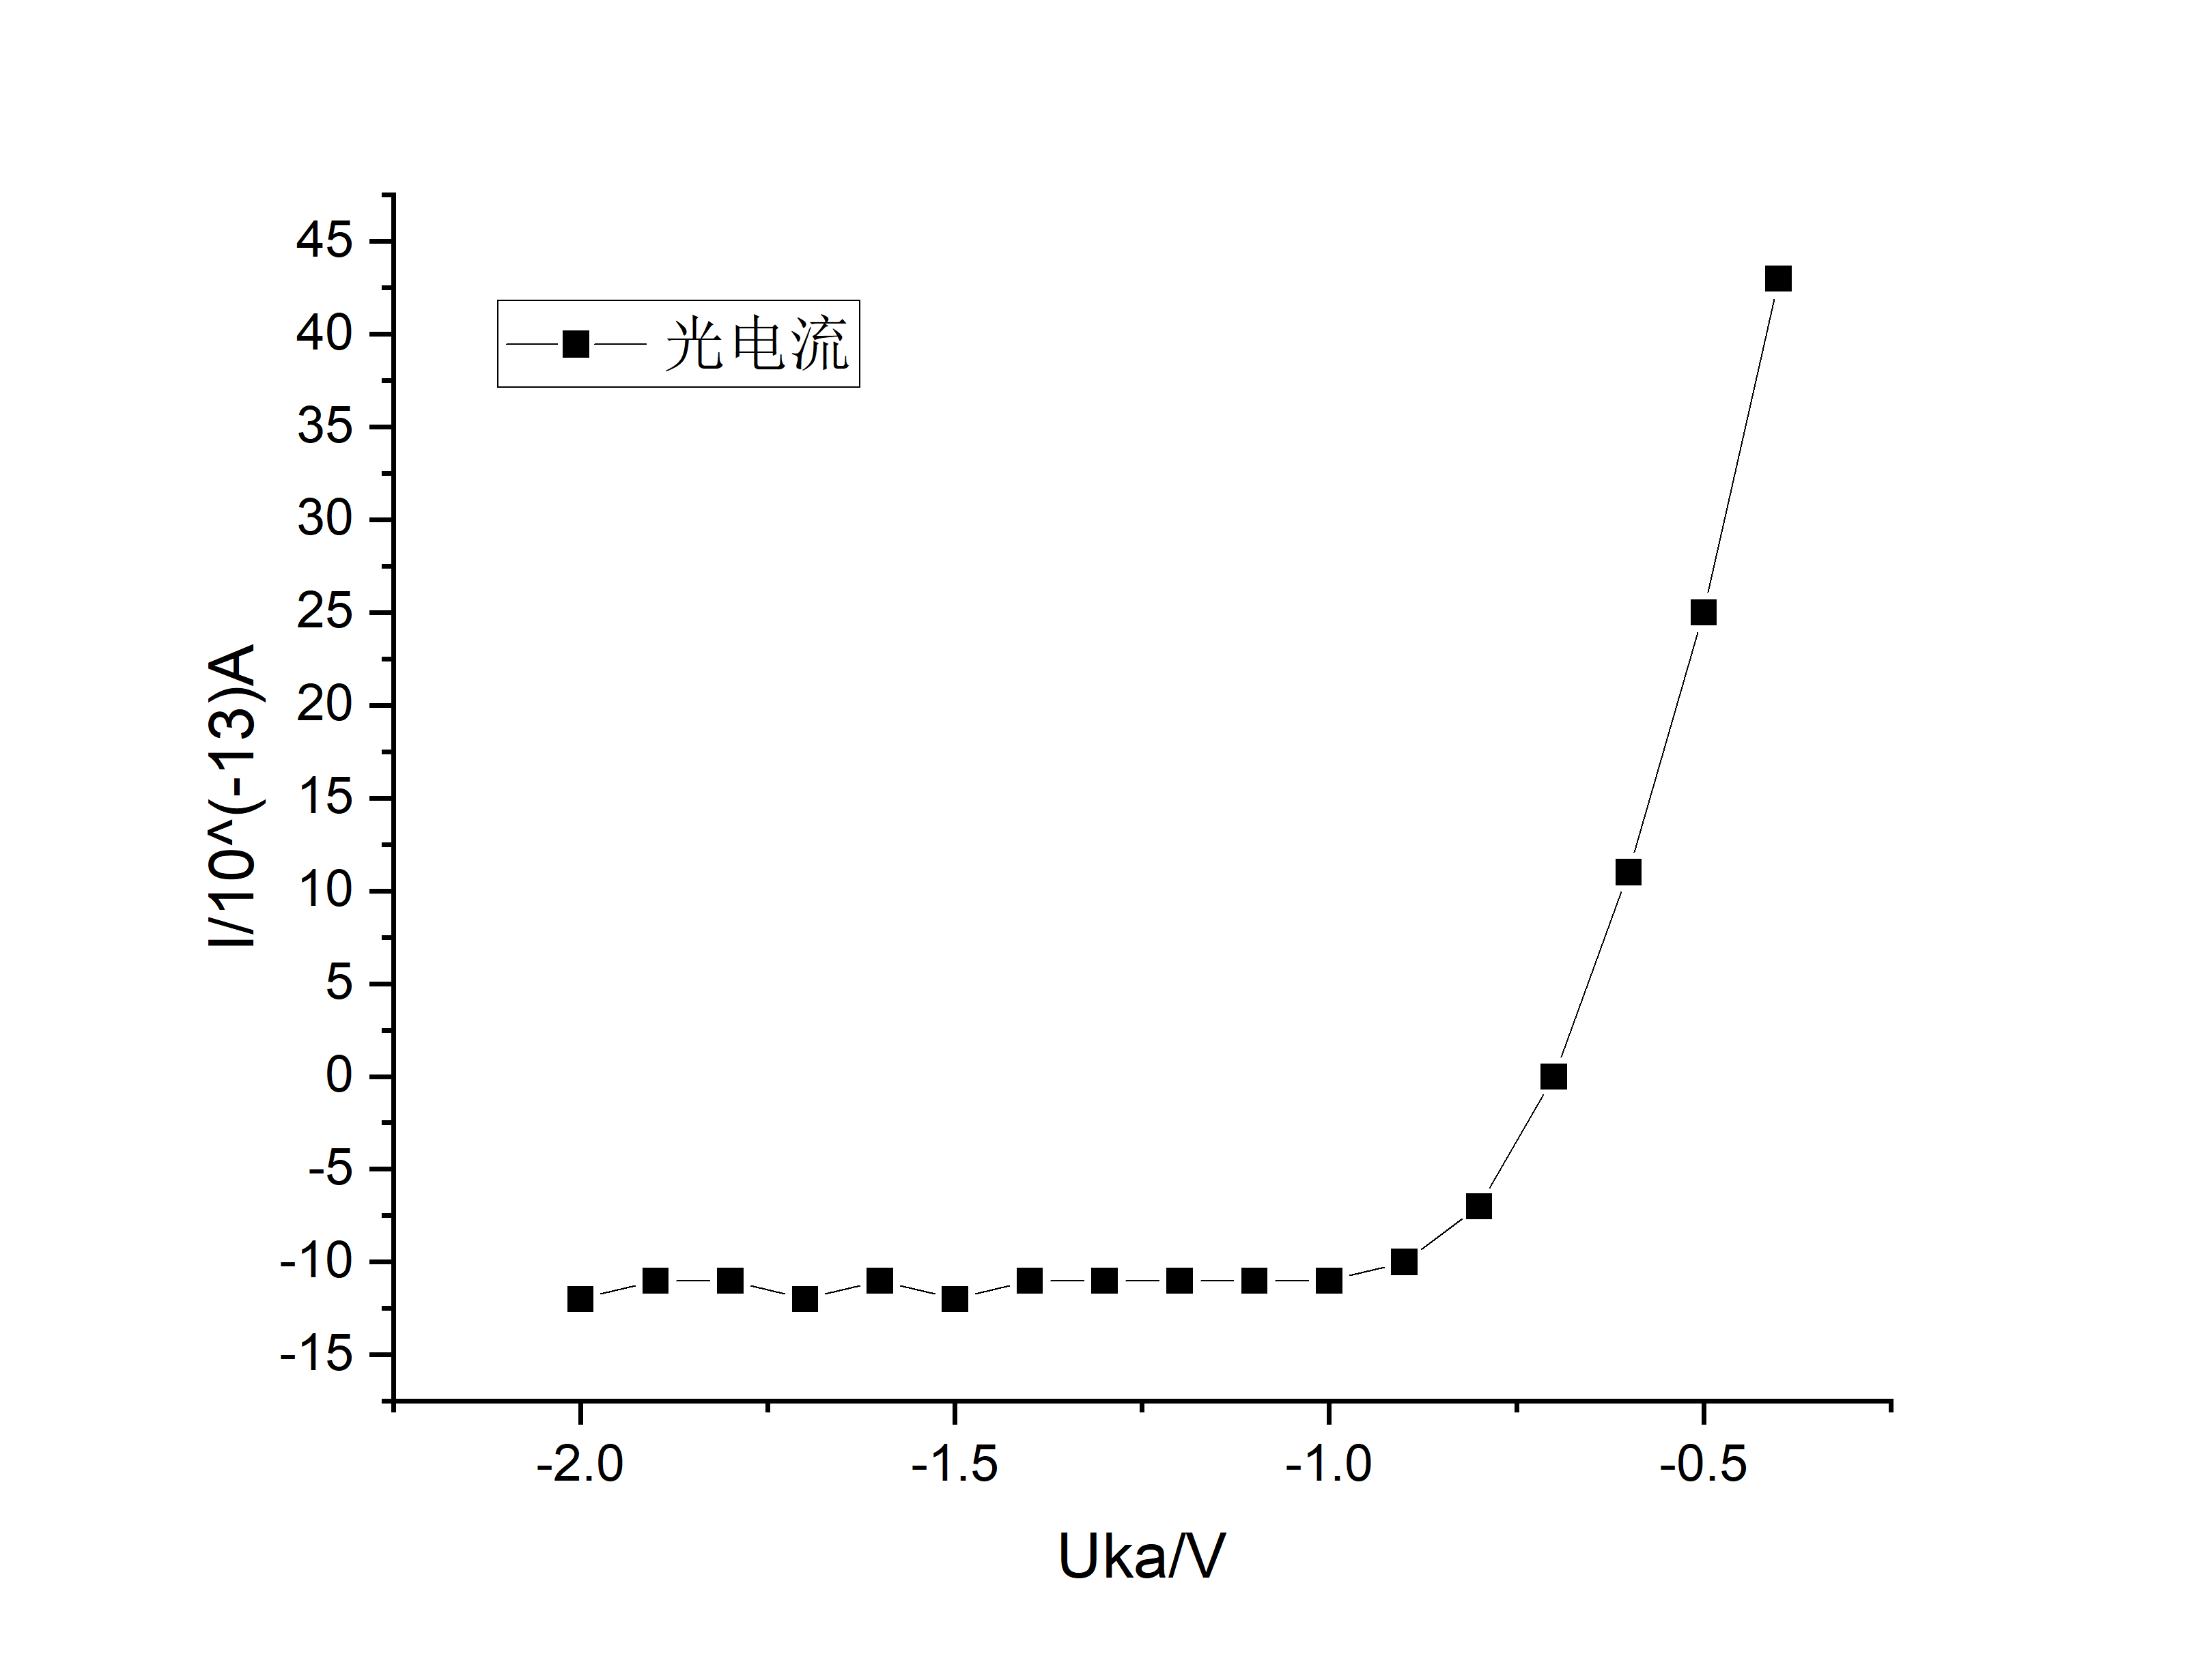
\includegraphics[width=0.33\textwidth]{img//546.png}
	}
	\subfloat[$\lambda=577nm$]{\label{fig:577}
	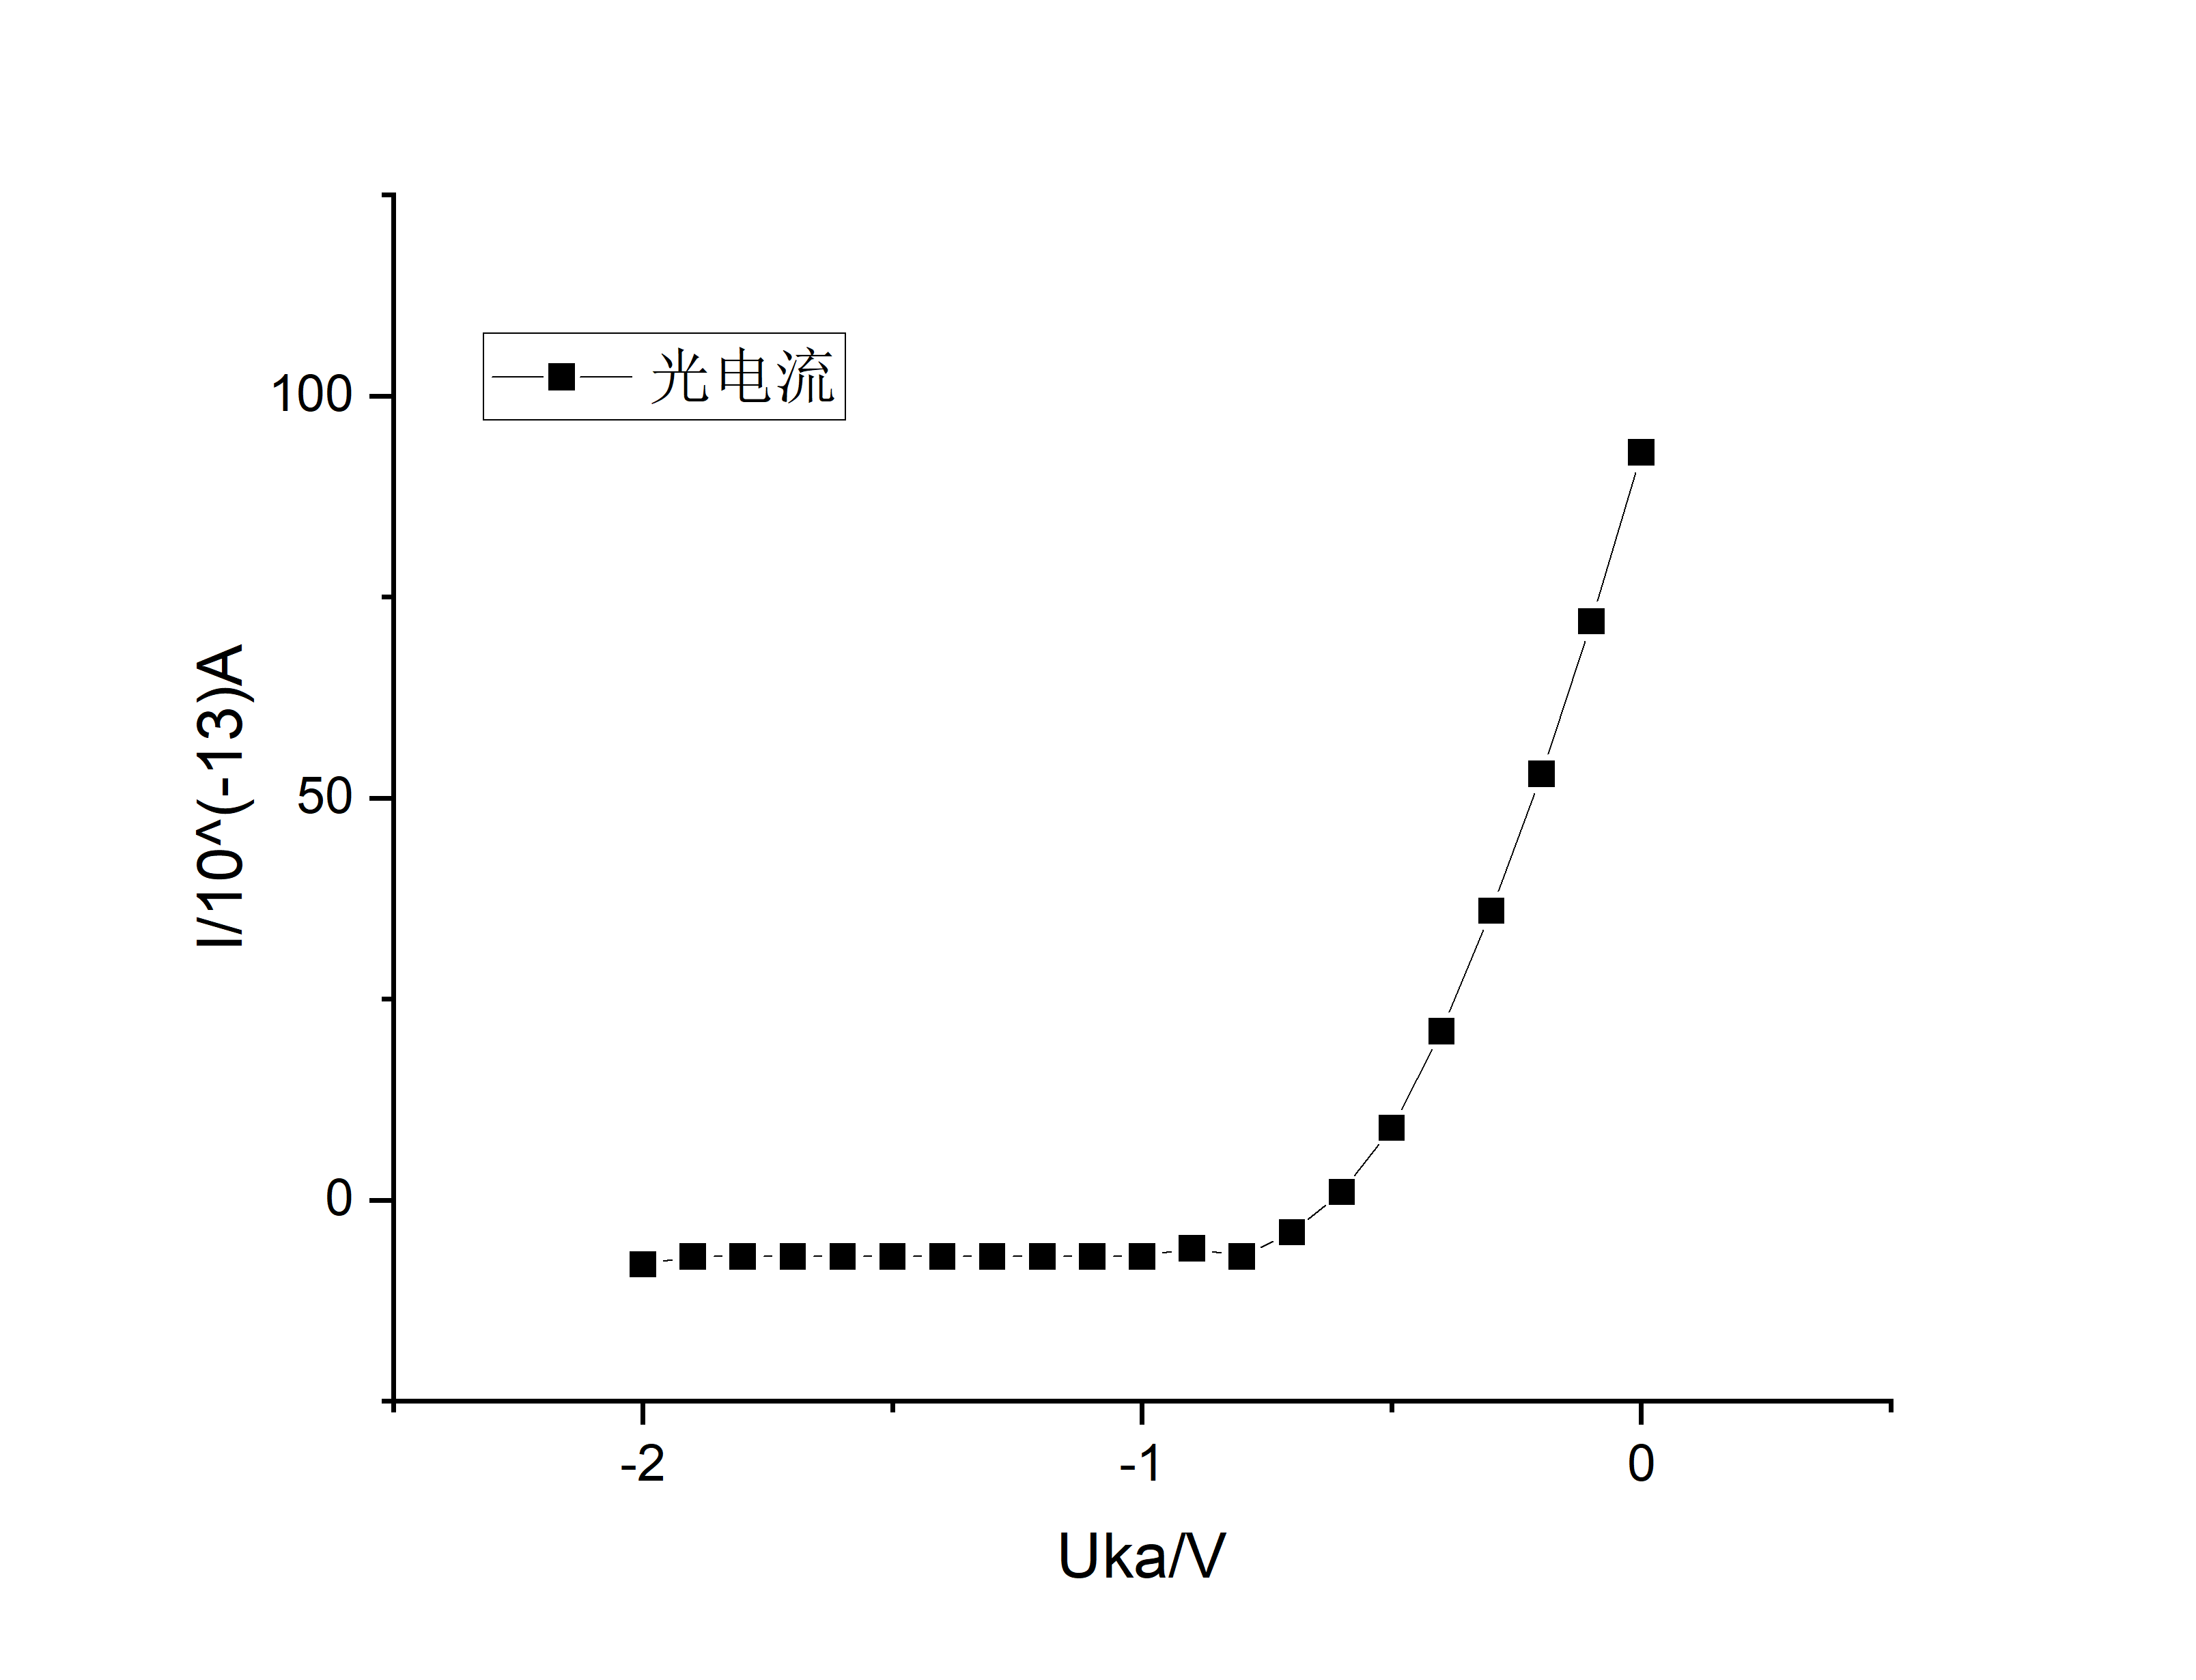
\includegraphics[width=0.33\textwidth]{img//577.png}
	}
	\caption{不同光谱光电流随$U_{KA}$变化关系曲线}
	\label{fig:2}
\end{figure}

由图\ref{fig:2}可以看出波长为365nm、405nm、436nm、546nm、577nm光谱光电流随$U_{KA}$变化关系曲线,图中的拐点称为抬头点。

首先由于光电管在加工制作和使用过程,阳极常会被溅射上光阴极材料,当光照射光阴极时,不可避免有部分光漫反射到阳极上,致使阳极也发射光电子,而外加反向电场对阳极发射的光电子成为一个加速场,它们很快到达阳极形成反向电流。

其次光电管即使没有光照,在外加电压下也会有微弱电流通过,称为光电管的暗电流。产生暗电流的主要原因是极间绝缘电阻漏电(包括管座及玻璃壳内外表面的漏电)和阴极在常温下的热电子发射,暗电流与加电压基本上成线性关系。

由于上述原因的影响,实测的光电流实际上是阴极光电子发射形成的光电流、阳极光电子发射形成的反向电流和光电管暗电流的代数和。
因此,真正的截止电压$U_s$并不是曲线与U轴的交点,因为此时阴极光电流并未截止。
当反向电压继续增大时,伏安特曲线将向反向电流继续延伸,达到抬头点时逐渐趋向饱和。
抬头点所对应的电压才是对应频率$\nu $下的截止电压。

数据处理时由于波长为365nm时抬头点不明显,故不计入表\ref{tab:1}.


\begin{table}[htbp]
	\centering
	\caption{不同波长光源饱和光电流数据}
	\vspace{0.7em}
	\resizebox{0.6\textwidth}{11mm}{ %第一个大括号为宽度,第二个大括号为高度(60mm)可随机设置,调整到适合该表格的大小为止
	\begin{tabular}{ccccc}
	\toprule
	光谱波长/nm & 405 & 436 & 546 & 577  \\
	\midrule
	频率/$10^{-14}Hz$ & 5.49 & 6.88 &  7.40 & 8.21\\
	$U_{KA}/V$ & -1.6 &-1.45 & -0.9 & -0.7\\
	\bottomrule
    \end{tabular}}%注意这里还有一个半括号
\label{tab:1}%
\end{table}


\begin{figure}[!h]
	\centering
	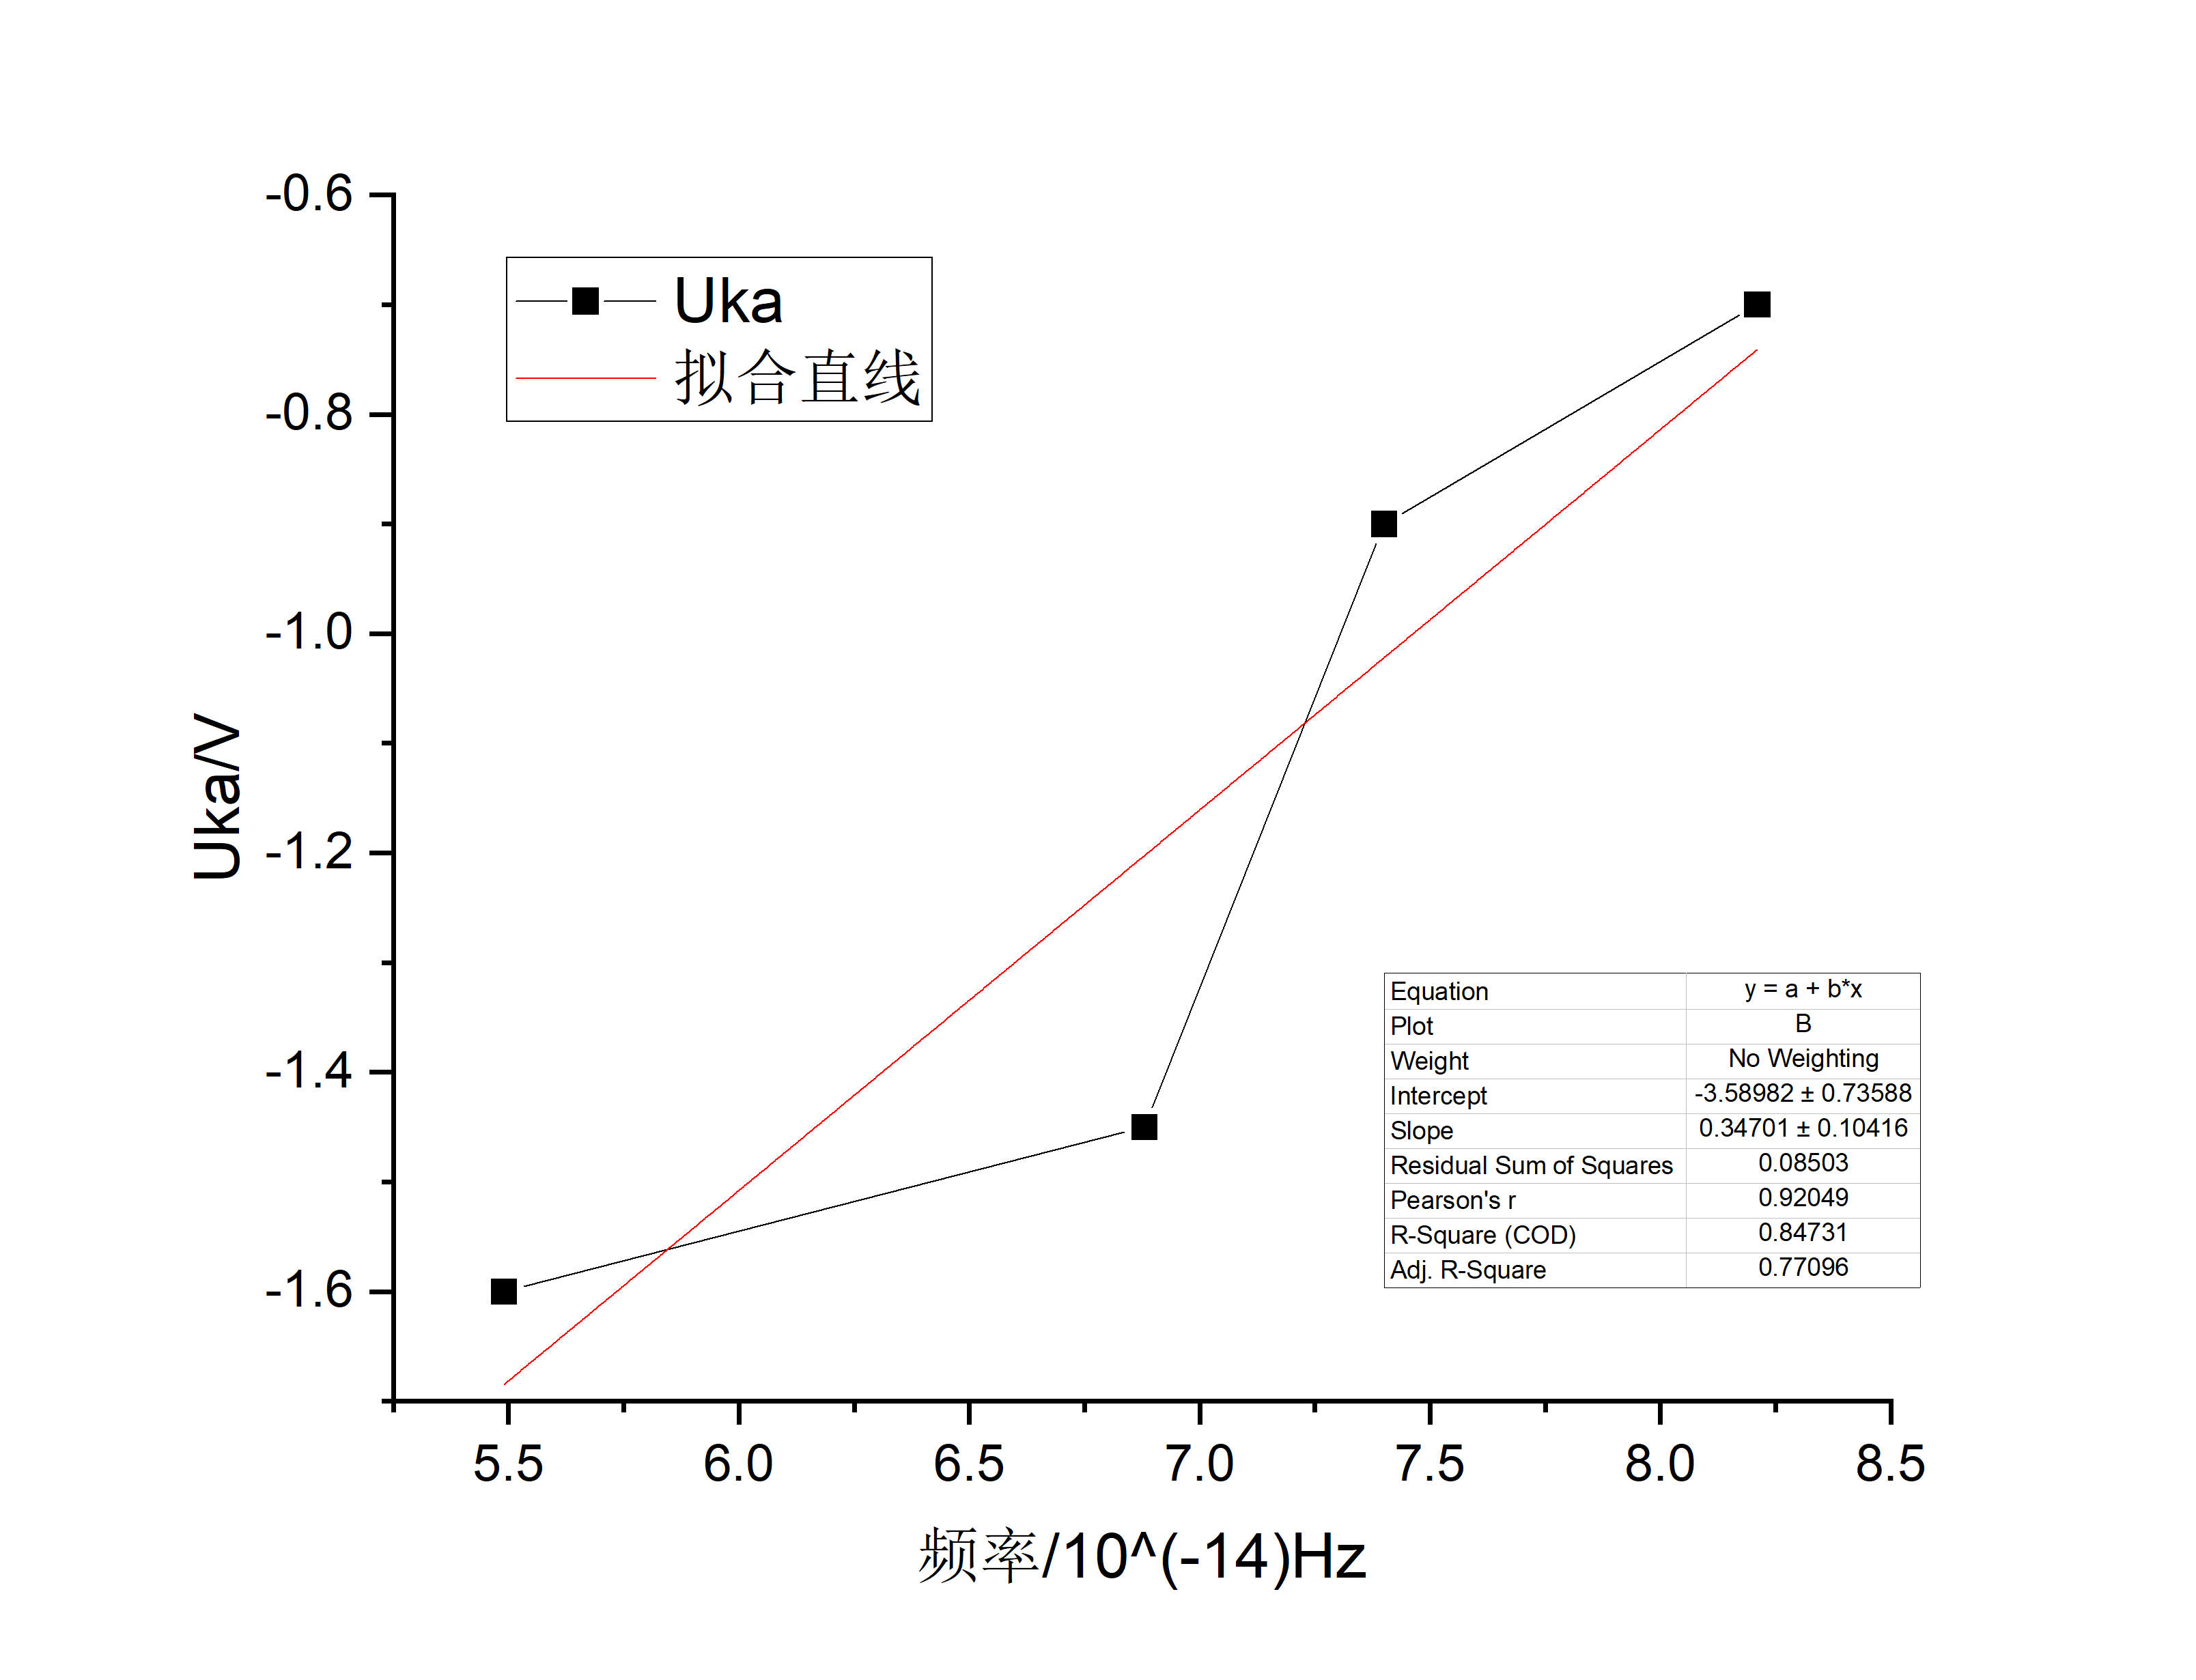
\includegraphics[width=0.6\textwidth]{img//reg2.png}
	\caption{截止电压随光源频率的变化曲线}
	\label{fig:3}
\end{figure}


相似的,线性拟合得斜率$k=0.3470\times 10^{-14}$,
同理可求得普朗克常数:
\begin{equation*}
	h=ke=5.56\times10^{-34} J \cdot s
\end{equation*}
计算相对误差E:
\begin{equation*}
	E=\frac{\left\lvert h-h_0\right\rvert }{h_0}\times 100\%=16.1\%
\end{equation*}

相对误差计算得知,零电流法比抬头点法测量结果更精确。通过线性拟合图也能得出,零电流法相关系数为0.99,而抬头点法为0.84,
零电流法更具线性。原因如下:

\begin{enumerate}
	\item 抬头点法测量步长过大,不能精确找到拐点,且人工找点本身就有较大偏差
	\item 零点相比于拐点更容易判别
	\item 抬头点法由于拐点不明显剔除一组数据,采样点较少导致偏差
\end{enumerate}

\subsection*{二、测量光电管的伏安特性曲线}
\subsubsection*{1.不同谱线在同一光阑,同一距离下的伏安饱和特性曲线}
实验参数:光源距离d=40mm,光阑直径$\phi=4mm$.

\begin{figure}[!h]
	\centering
	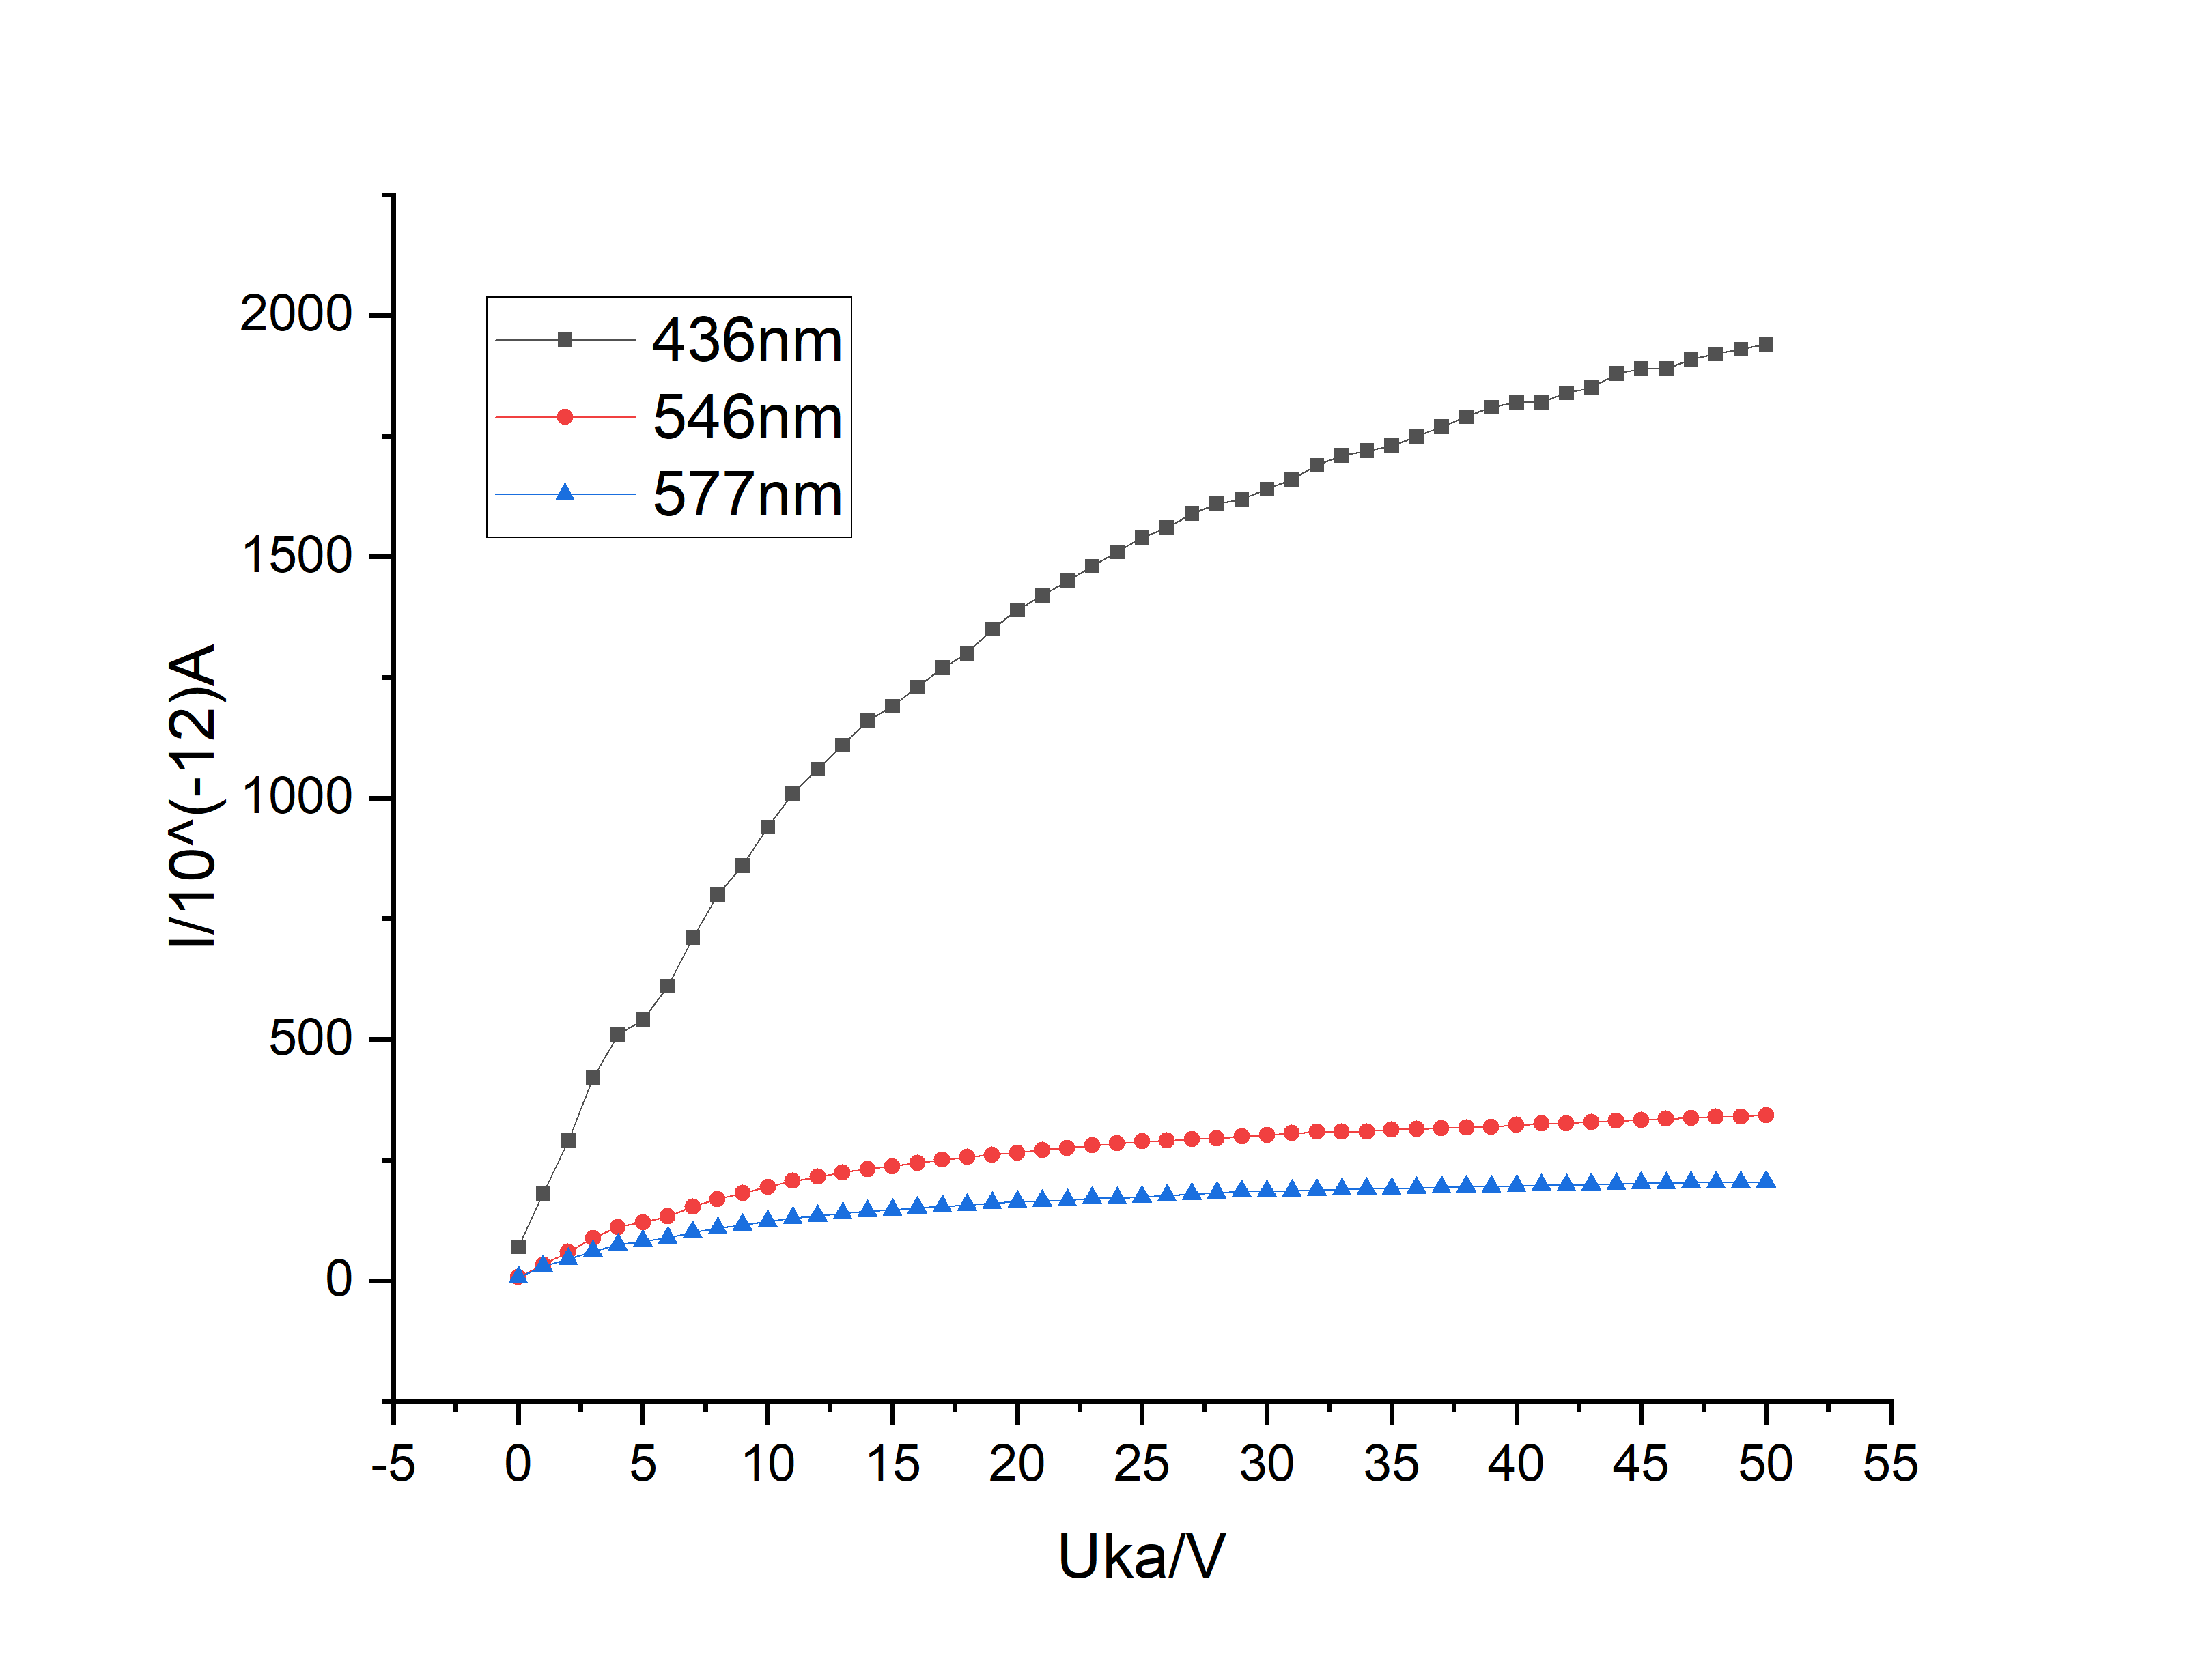
\includegraphics[width=0.6\textwidth]{img//lambda.png}
	\caption{不同谱线伏安饱和特性曲线}
	\label{fig:lambda}
\end{figure}

图\ref{fig:lambda}可见在接近50V电压时电流增大开始逐渐放缓,可以将50V电压对应光电流近似为饱和光电流:

\begin{table}[htbp]
	\centering
	\caption{不同波长光源抬头点数据}
	\vspace{0.7em}
	\resizebox{0.5\textwidth}{8mm}{ %第一个大括号为宽度,第二个大括号为高度(60mm)可随机设置,调整到适合该表格的大小为止
	\begin{tabular}{ccccc}
	\toprule
	光谱波长$\lambda/nm$ & 436    & 546 & 577  \\
	\midrule
	饱和电流$I_M/10^{-12}A$   & 1940  &  343 & 204\\
	\bottomrule
\end{tabular}}%注意这里还有一个半括号
\label{tab:2}%
\end{table}

由表\ref{tab:2}可得在同一光阑、同一距离下,波长越短,频率越高,饱和光电流越大。

\subsubsection*{2.某条谱线,同一光阑,不同距离下的伏安饱和特性曲线}
已知光强与光源距离的平方成反比,故不同距离可看成不同光强下的伏安饱和特性曲线。

实验参数:光源波长$\lambda=436nm$,光阑直径$\phi=4mm$.

\begin{figure}[!h]
	\centering
	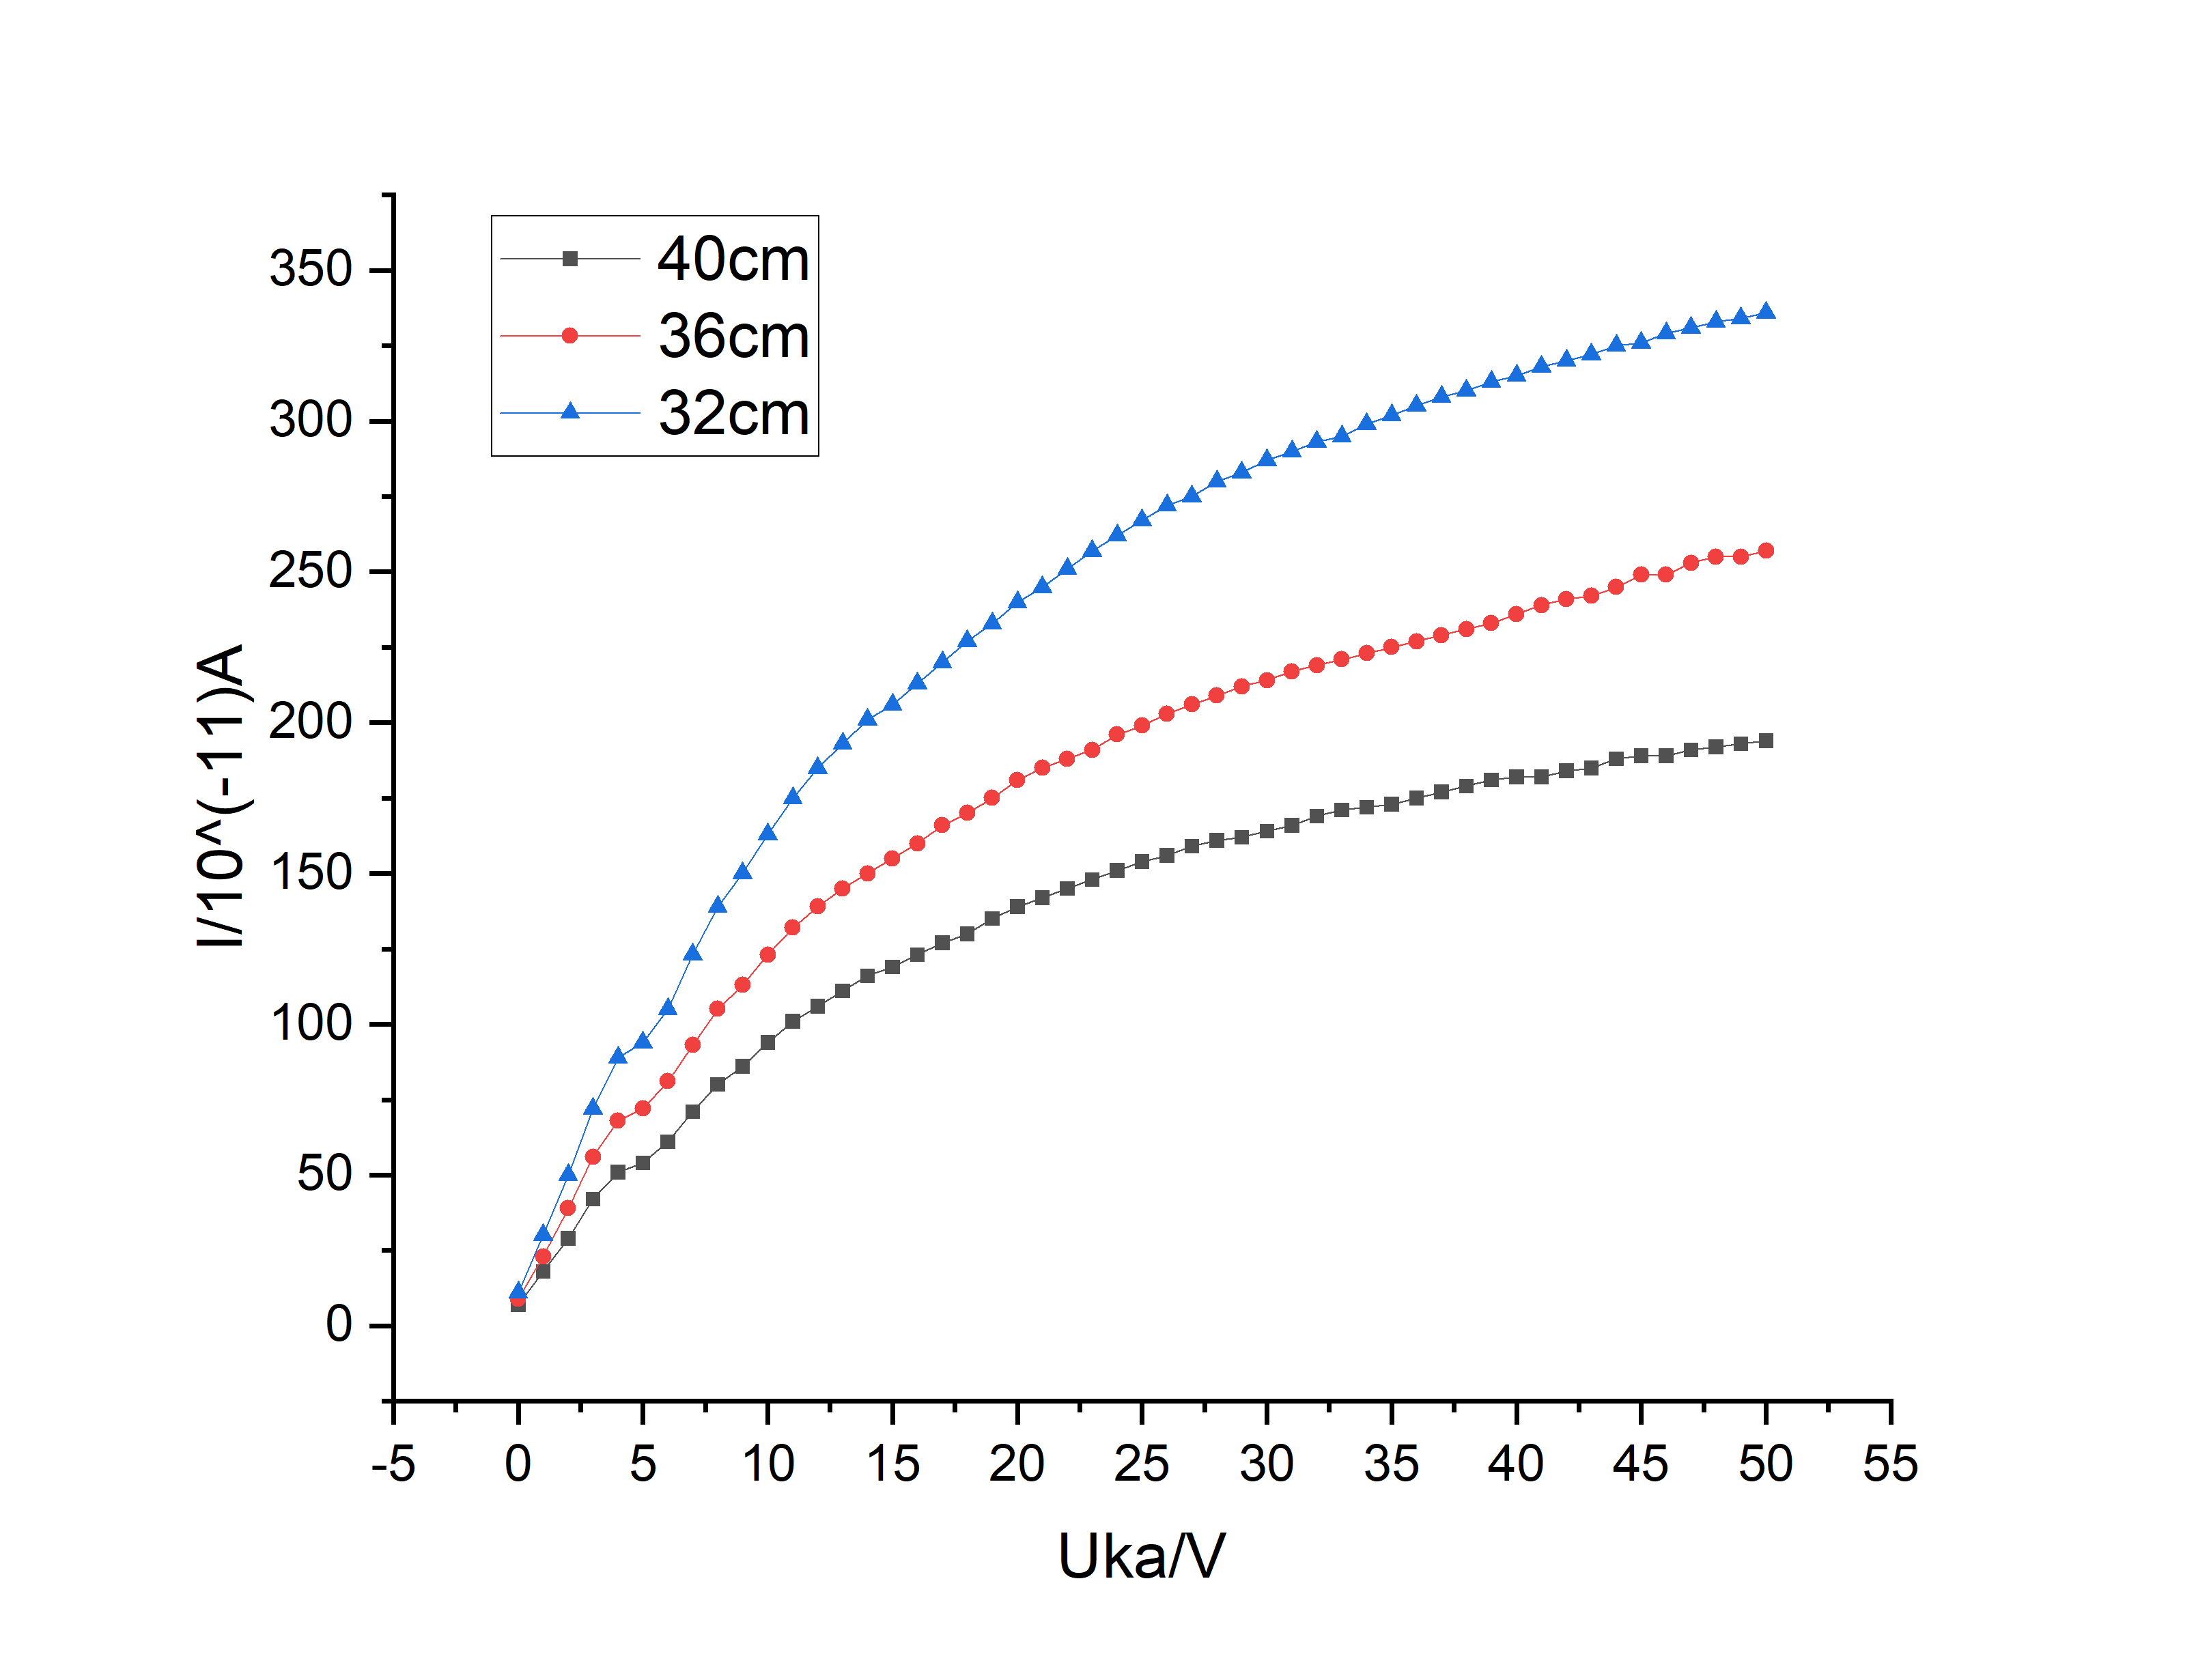
\includegraphics[width=0.6\textwidth]{img//d.png}
	\caption{不同光强伏安饱和特性曲线}
	\label{fig:d}
\end{figure}

图\ref{fig:d}可见在接近50V电压时电流增大开始逐渐放缓,可以将50V电压对应光电流近似为饱和光电流:
\begin{table}[htbp]
	\centering
	\caption{不同光强饱和电流值}
	\vspace{0.7em}
	\resizebox{0.5\textwidth}{11mm}{ %第一个大括号为宽度,第二个大括号为高度(60mm)可随机设置,调整到适合该表格的大小为止
	\begin{tabular}{ccccc}
	\toprule
	光源距离d/cm & 32    & 36 & 40  \\
	\midrule
	$d^{-2}/10^{-4}\times(cm)^{-2}$    &  9.77 &  7.71 &6.25\\
	饱和电流$I_M/10^{-11}A$      & 336    &  257 & 194\\
\bottomrule
\end{tabular}}%注意这里还有一个半括号
\label{tab:3}%
\end{table}

由表\ref{tab:3}可得在同一波长、同一光阑下,距离越短,光强越大,饱和光电流越大。


作饱和光电流随距离平方反比(正比于光强)的变化曲线,如图\ref{fig:4}
\begin{figure}[!h]
	\centering
	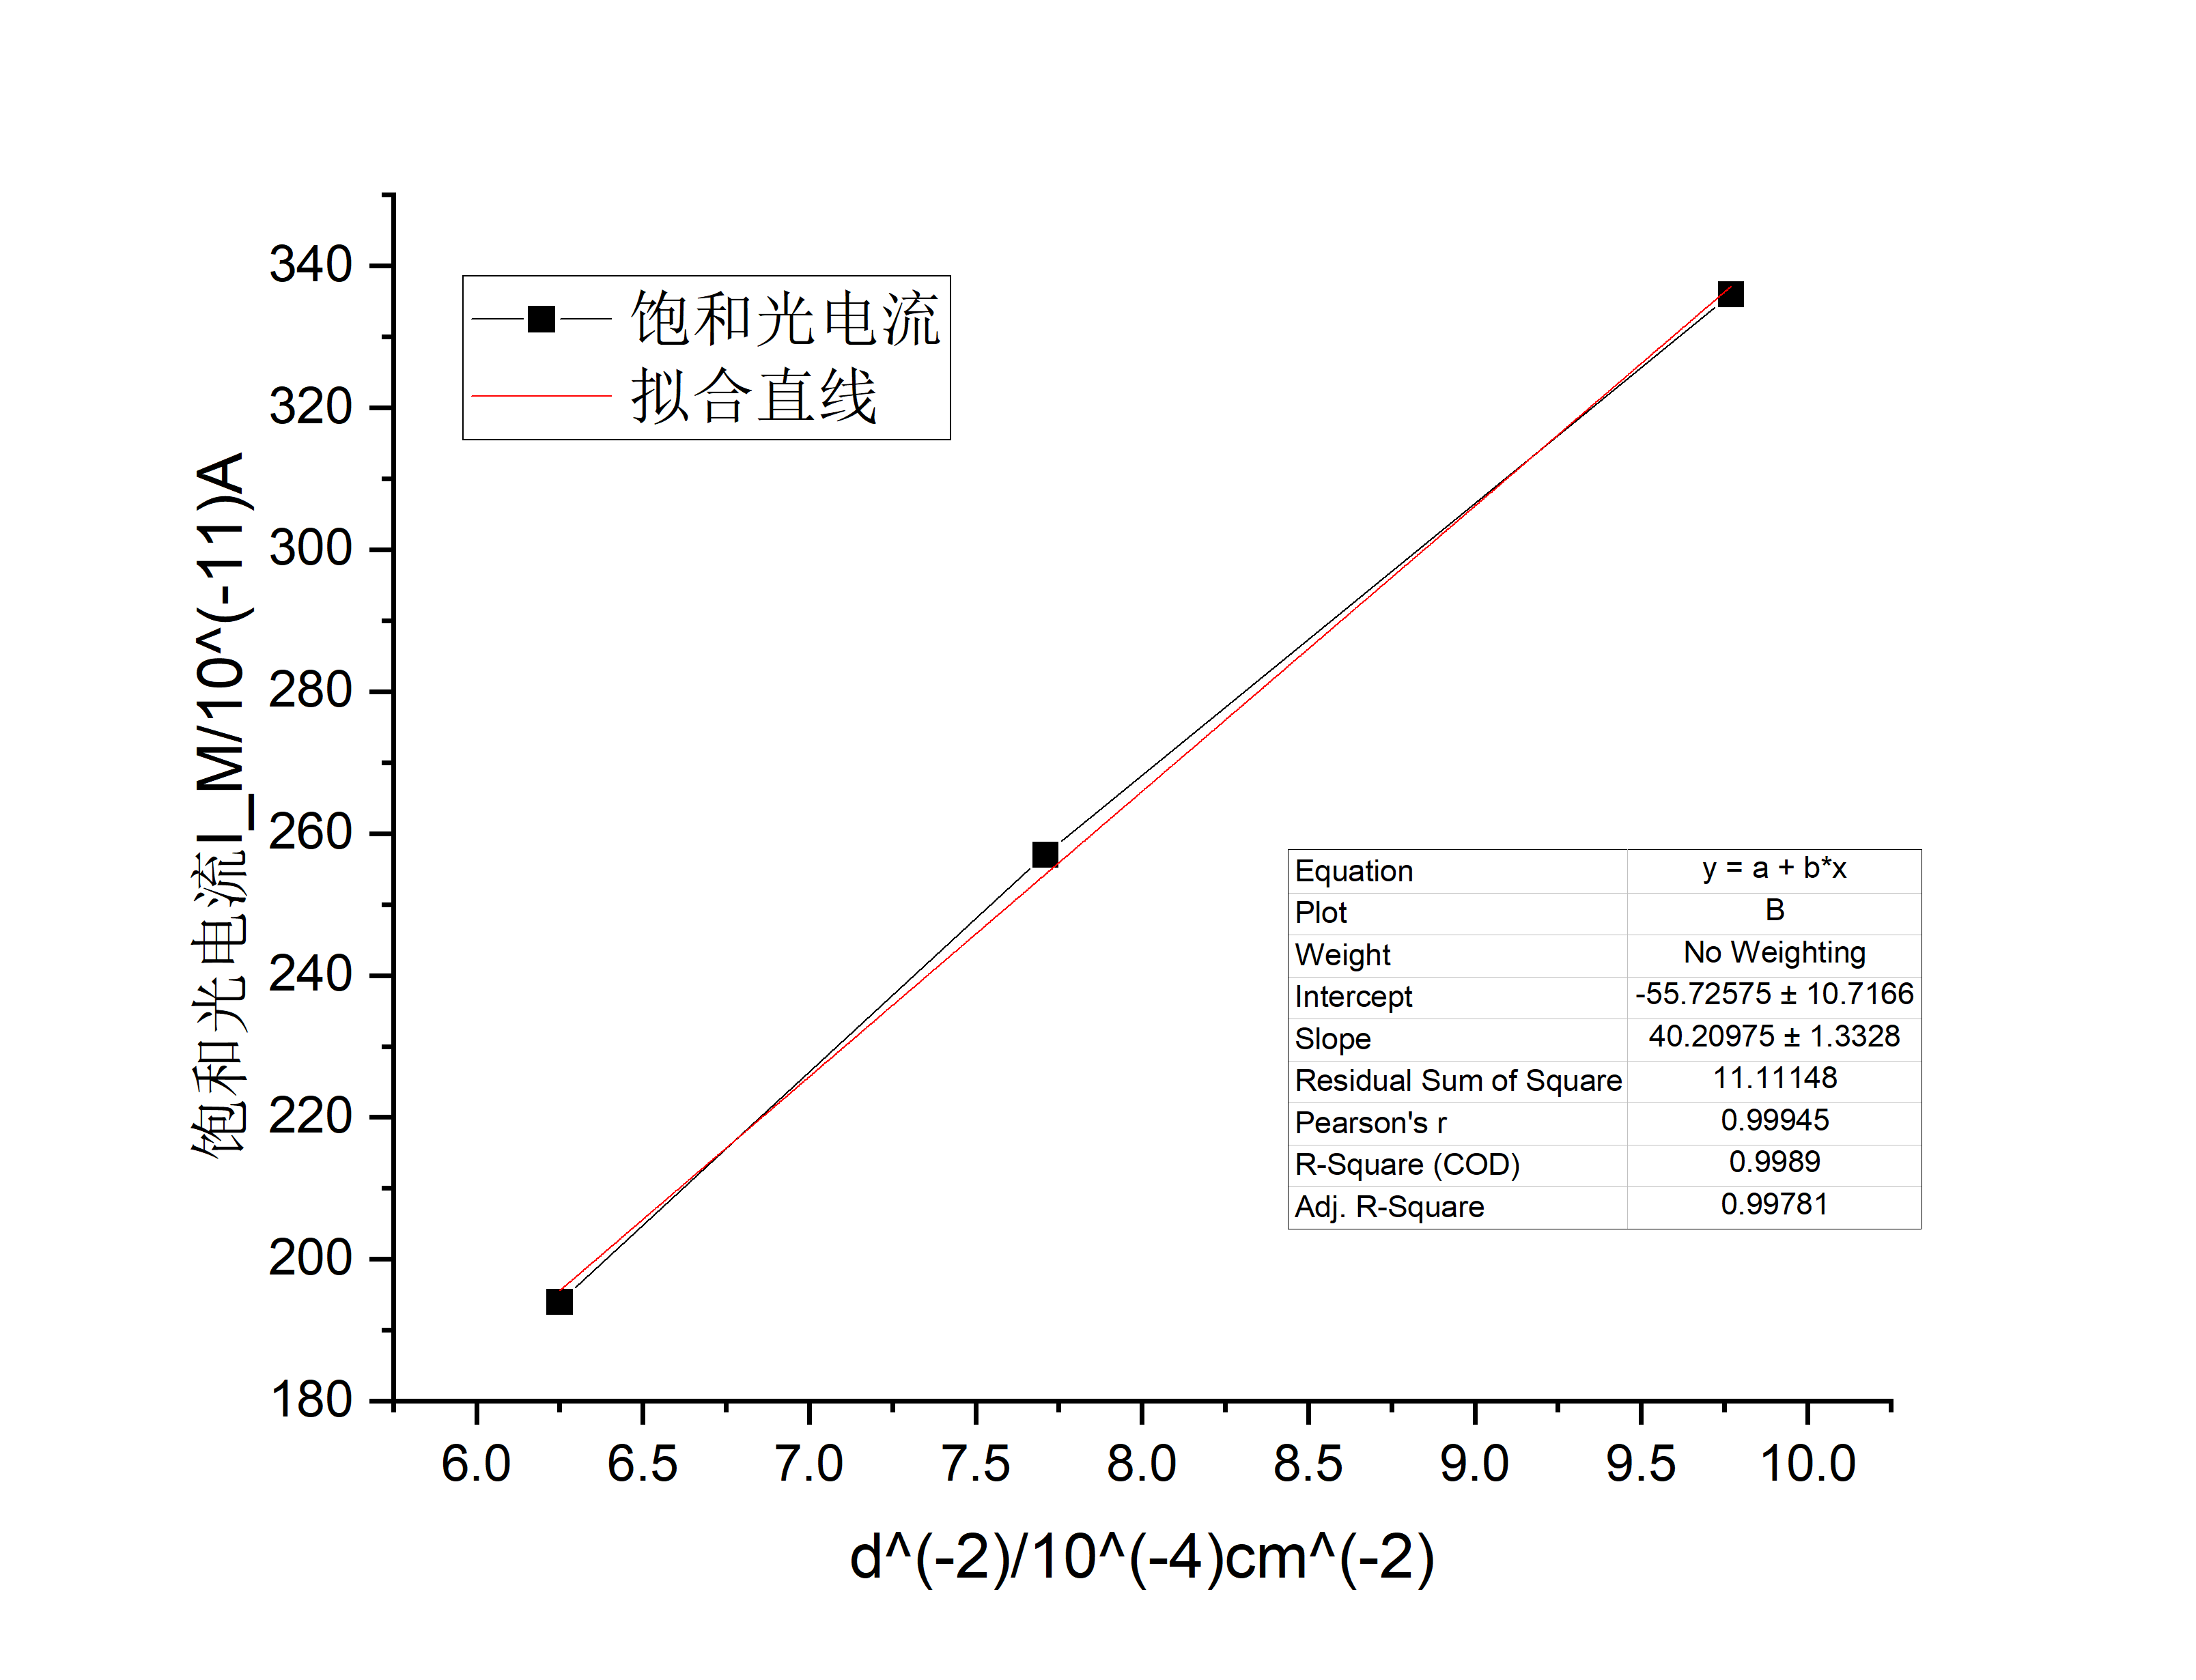
\includegraphics[width=0.6\textwidth]{img//reg3.png}
	\caption{光电流随距离平方反比的变化曲线}
	\label{fig:4}
\end{figure}
结论:由图\ref{fig:4},,拟合曲线相关系数为0.99,在误差允许的范围内,线性关系良好。
光电管的饱和光电流与光电管与光源之间的距离的平方成反比,与入射光强成正比。

\subsubsection*{3.同一谱线,同一距离,不同光阑下的伏安饱和特性曲线}
实验参数:光源波长$\lambda=436nm$,光源距离$\lambda=40cm$.

\begin{figure}[!h]
	\centering
	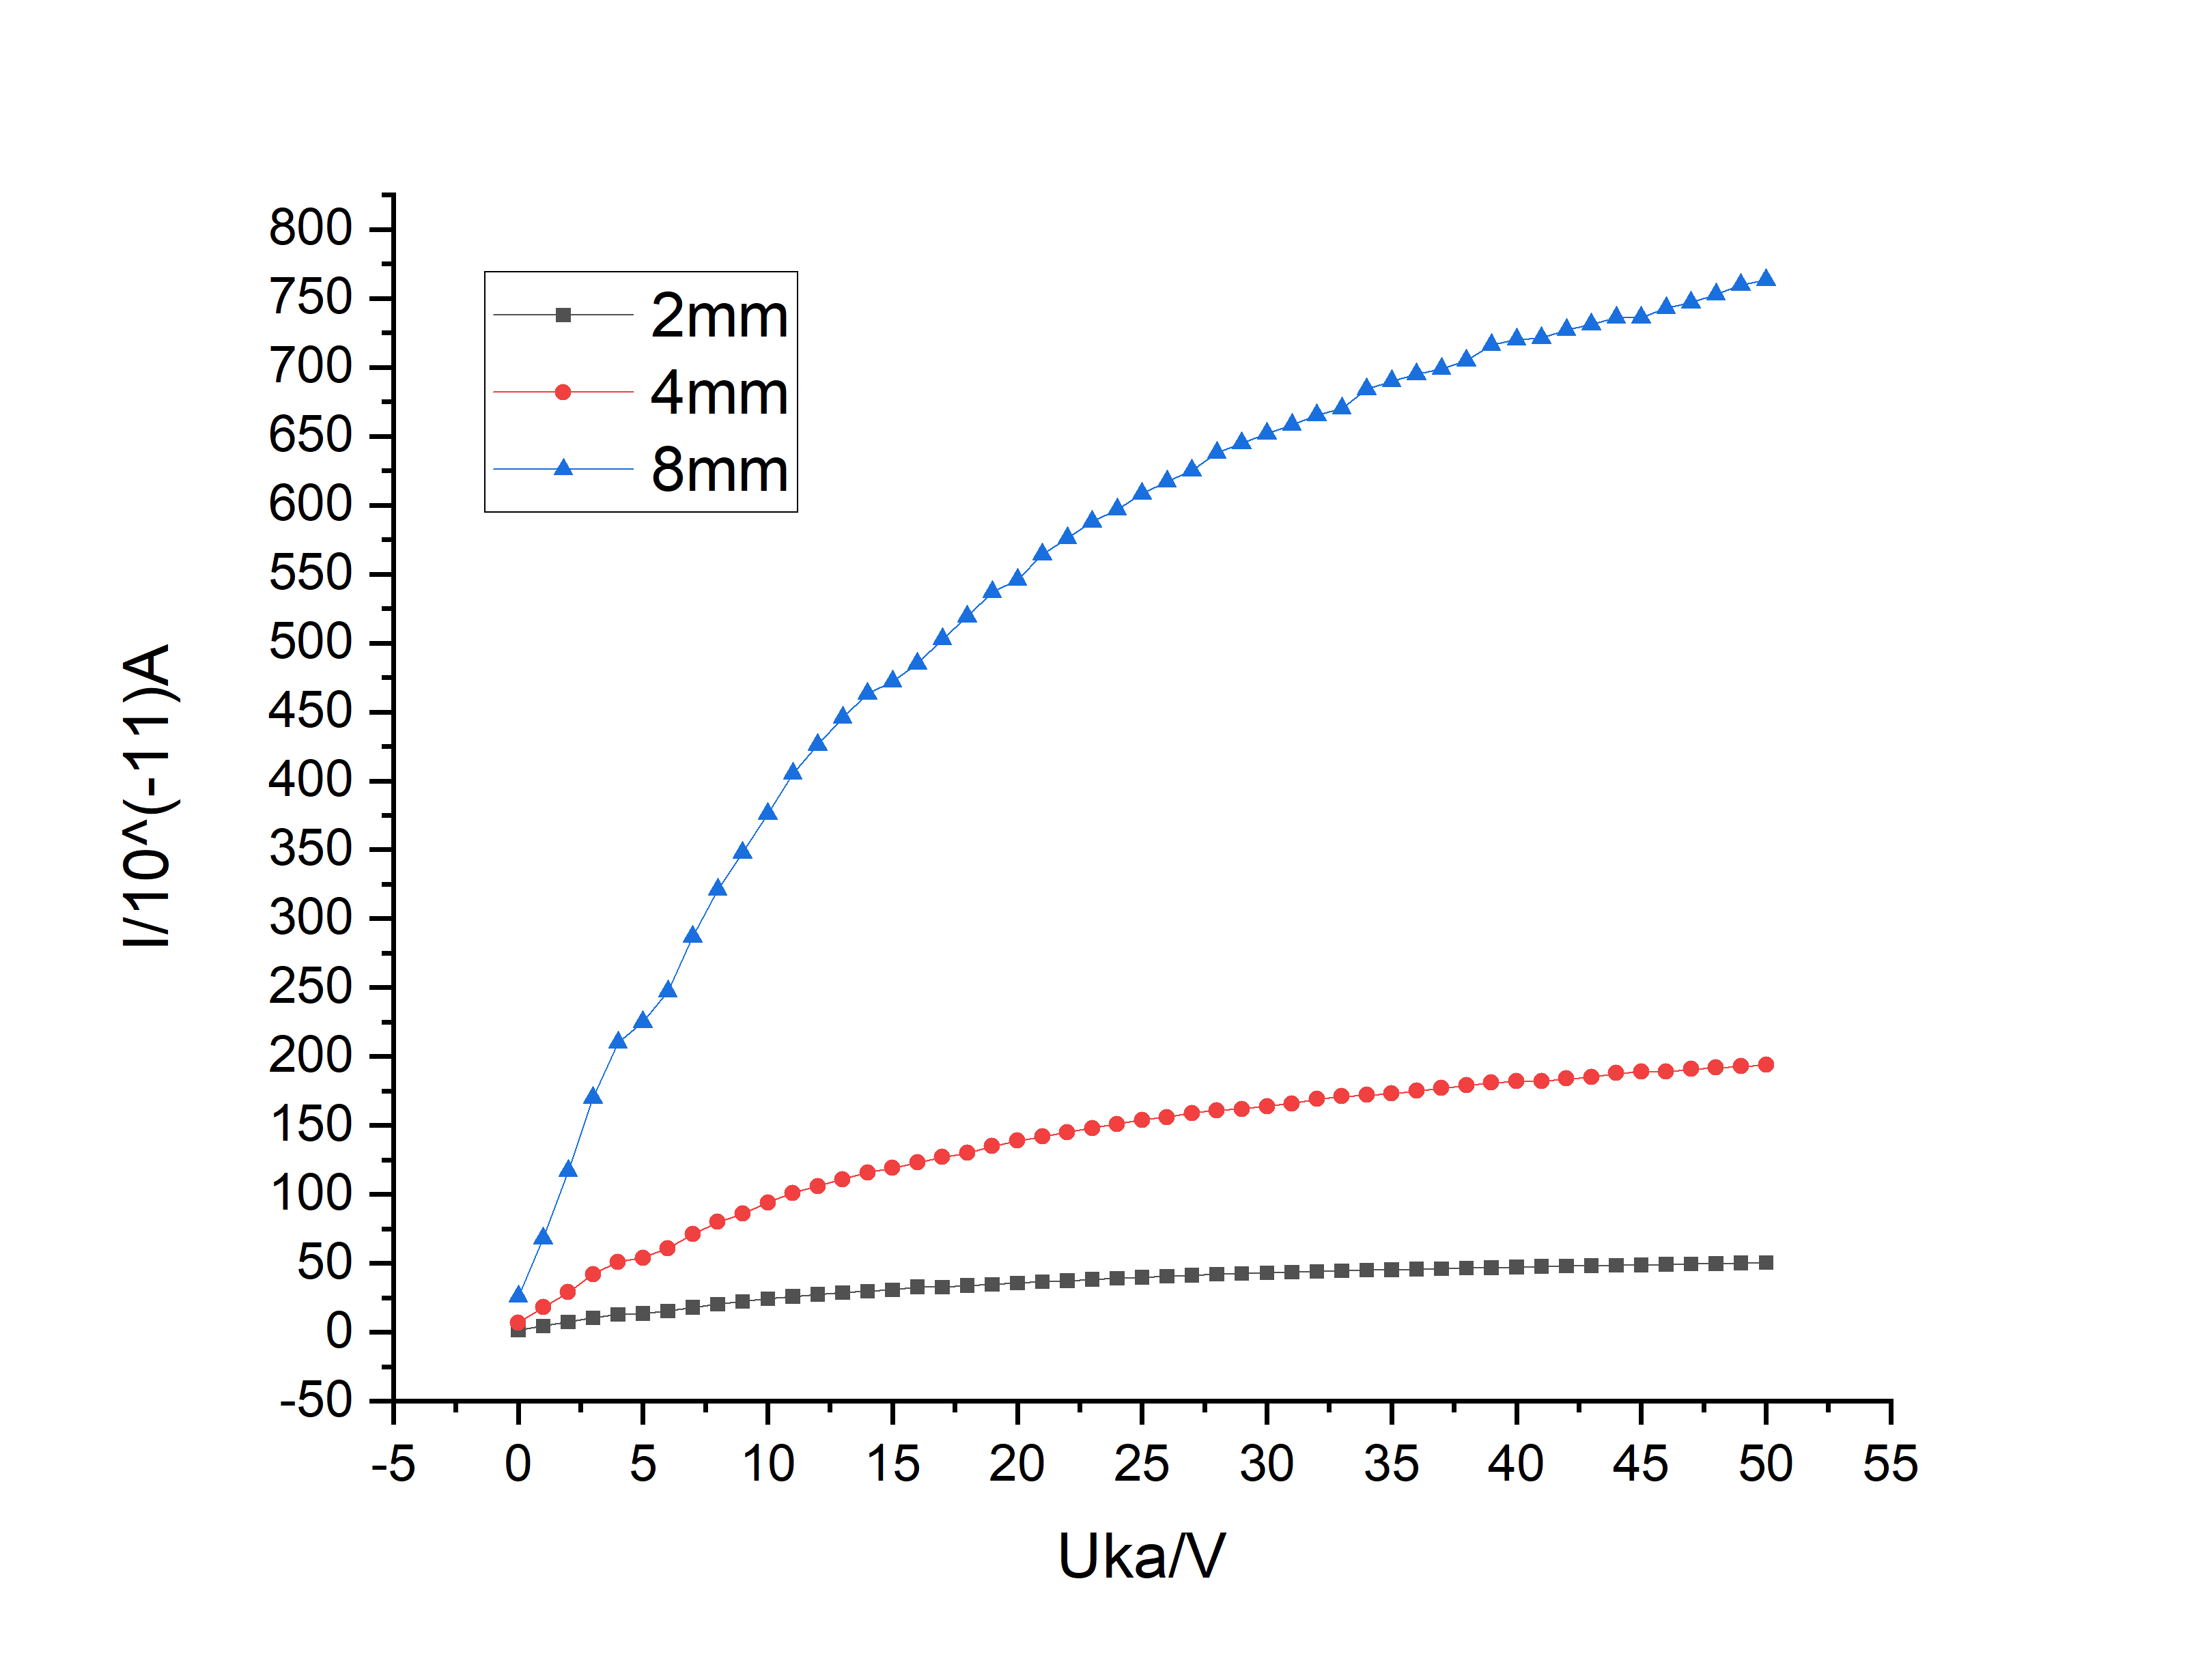
\includegraphics[width=0.6\textwidth]{img//phi.png}
	\caption{截止电压随光源频率的变化曲线}
	\label{fig:phi}
\end{figure}
图\ref{fig:phi}可见在接近50V电压时电流增大开始逐渐放缓,可以将50V电压对应光电流近似为饱和光电流:

\begin{table}[htbp]
	\centering
	\caption{不同直径光阑饱和电流值}
	\vspace{0.7em}
	\resizebox{0.5\textwidth}{9mm}{ %第一个大括号为宽度,第二个大括号为高度(60mm)可随机设置,调整到适合该表格的大小为止
	\begin{tabular}{ccccc}
	\toprule
	光阑直径$\phi/mm$ & 2  & 4 & 8  \\
	\midrule
	饱和电流$I_M/10^{-11}A$  & 50.5 &  194 & 763\\
\bottomrule
\end{tabular}}%注意这里还有一个半括号
\label{tab:4}%
\end{table}

由表\ref{tab:4}可得在同一波长、同一距离下,光阑孔径越大,光强越大,饱和光电流越大。

作饱和光电流随光阑直径的变化曲线,如图\ref{fig:5}
\begin{figure}[!h]
	\centering
	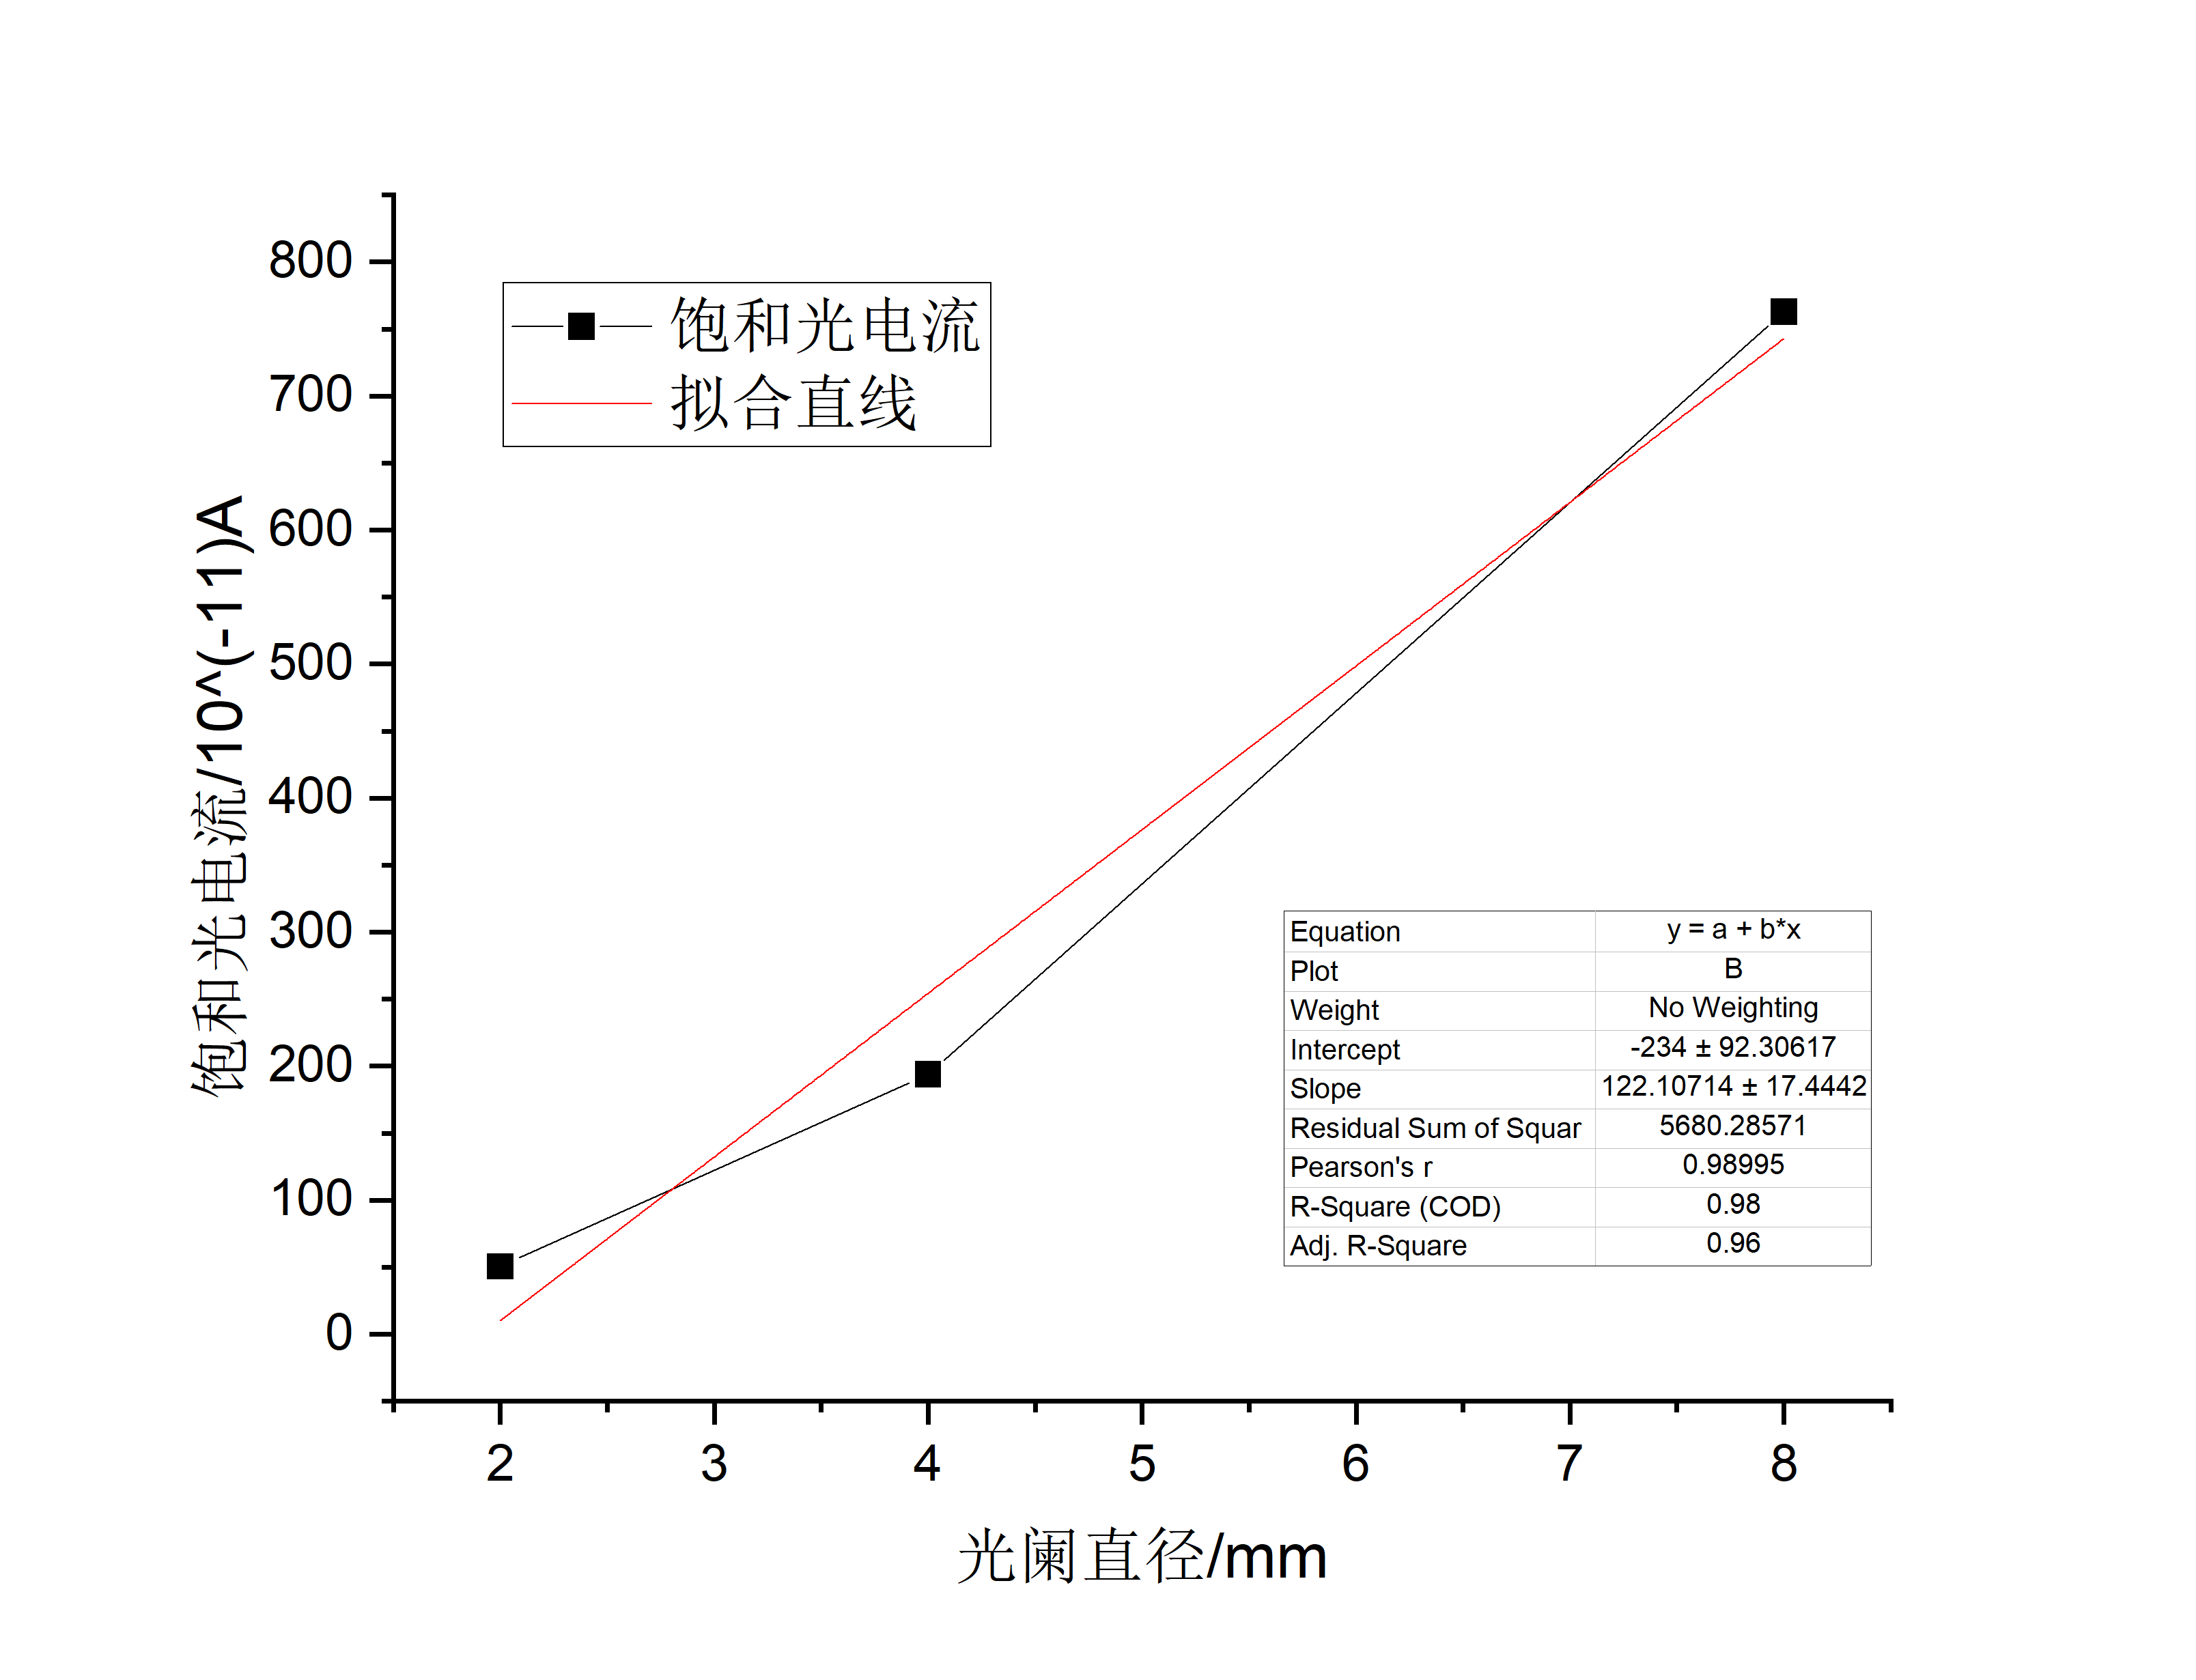
\includegraphics[width=0.6\textwidth]{img//reg4.png}
	\caption{光电流随光阑直径的变化曲线}
	\label{fig:5}
\end{figure}
结论:由图\ref{fig:5},,拟合曲线相关系数为0.98,在误差允许的范围内,线性关系良好。
光阑孔径可看成与光强成正比,光电管的饱和光电流与光阑孔径大小成正比,即与入射光强成正比。

\subsubsection*{【误差分析】}
\begin{enumerate}
	\item 仪器本身的误差。在测量读数时,最后一位有效数字常常变化,使读数有一定的误差。有时三路线性直流电源输入的电压也不稳定,也产生一定的误差。
	\item 滤光片的镜片由于长时间使用,滤光的效果有一定的影响。
	\item 周围的电灯光线使进入光电管的光强有一定的误差。
	\item 零电流法的误差。阳极反向电流的存在使得电流零点不是阴极电流为零,而是阴极与阳极电流的代数和为零。
\end{enumerate}

\section*{【思考题】}
\subsubsection*{1.截止电压的物理意义是什么?}
答:光子照射到光电管的阴极,电子吸收光子的能量 ,使自身能量增加。
当电子吸收的能量足够大,能够克服脱离物体表面的逸出功时,电子就可以离开阴极表面脱逸出来,成为光电子。
由于光电子具有初动能,即使阳极不加电压也会有光电子从阴极逸出到阳极形成光电流,甚至阳极相对于阴极的电位低时也会有光电子落入阳极,直到阳极电位低于某一数值时,所有光电子都不能达到阳极,光电流才为零。
这个使光电流为零的相对于阴极为负的负方向电压U称为光电效应的截止电压。
\subsubsection*{2.实验仪选择不同的电流灵敏度(即不同的电流测量档)是否会影响普朗克常数的测量结果?}
答:不同的电流灵敏度会影响普朗克常量的测量结果。因为我们是取电流为零时对应的电压值为截止电压,并由各组电压与频率的数据做出图线求斜率,以斜率求普朗克常量。
假如电流的灵敏度较小,电压值与真实截止电压相差就较大。
如果选择的电流测量挡过大,仪表显示的电流零点会有不止一个,在电压的一个小区间内电流都会显示为零,这就大大降低了测量的精确性,算出来的普朗克常量与公认值的相对误差也比较大。
\subsubsection*{3.光电管与光电池有什么区别?}
答:光电管是以光电效应原理产生光电子,通过光电子的定向运动产生电流的;而光电池是以半导体内光电效应为原理产生电位差,从而形成电流。
\subsubsection*{4本实验最大的误差来源是什么?试提出一些减少实验误差的建议。}
答:本实验误差来源主要是周围杂散光对实验的影响,杂散光照射光电管会使本底电流增大,使得用零电流法测得的截止电压与真实值差距增大。
为了减少实验误差,可设计一个遮光罩以排除外界光源对实验的影响。
在测伏安特性曲线实验中,在实际读数开始之前可以先大致观察一下在不同电压下电流的变化幅度,以选择最适合的电流测量档,可以有效减小测量误差。


\section*{【参考文献】}
\begin{enumerate}
	\item 沈韩.基础物理实验[M].科学出版社,2015.
	\item 吴立君,李倩.光电效应测普朗克常数的三种方法[J].大学物理实验,1007-2934(2007)-04-0049-04.
	\item 侯春,隋成华,徐来定,高建勋,陈磊.光电效应实验中的误差分析及消除方法[J].学仪器,2002(Z1):14-17.
	\item 刘敏敏.测量条件对普朗克常数的影响[J].大学物理实验,2015,28(05):86-90.
\end{enumerate}

\end{document}